\chapter{Lie theory and Jacobi diagrams}
\label{ch:lie-theory-and-jacobi-diagrams}

\lettrine{\libertineInitialGlyph{T}}{he} fundamental theorem of Vassiliev invariants states that the bialgebra of Vassiliev invariants can be broken up into ``nice'' combinatorial weight systems. So to understand \(\mathcal{V}\) it suffices to understand \(\mathcal{W}\) (or equivalently its dual \(\mathcal{A}\)). As we will see in this chapter, the structure of \(\mathcal{A}\) is related to Lie theory.

\section{Jacobi diagrams}
To see the Lie theory connections, we see that \(\mathcal{A}\) is isomorphic as a bialgebra of Jacobi diagrams, whose elements are represented by graphs with one- and three-valent vertices.

\begin{definition}
	A \textbf{unitrivalent diagram} is a unitrivalent graph (with loops and multiple edges allowed) with the following additional data:
	\begin{itemize}[topsep=0.3em, itemsep=-1pt]
		\item each trivalent vertex has a fixed cyclic order of incident edge-connections,
		\item the set of univalent vertices has a fixed cyclic order.
	\end{itemize}
	The vector space of unitrivalent diagrams is denoted \(\mathcal{T}\).
\end{definition}

\begin{warning}
	When drawing unitrivalent diagrams, there are two notational conventions we use. Firstly, the fixed cyclic order of the univalent edges is specified by drawing them connected to a circle (where the cyclic order corresponds to traversing the circle anticlockwise). Like for chord diagrams, this circle is called the \textbf{skeleton}. Secondly, the trivalent vertices are assumed to have the cyclic order corresponding to traversing anticlockwise around the vertex. It is always possible to draw them this way because planarity is not a concern of abstract graphs.
\end{warning}

In particular, all chord diagrams are unitrivalent diagrams with only univalent vertices (the chord ends). Further examples of unitrivalent diagrams would be
\[
	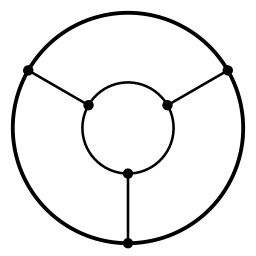
\includegraphics[width=0.13\textwidth, valign=c]{graphics/unitrivalent_diagram_example_1.pdf} \ ,
	\quad
	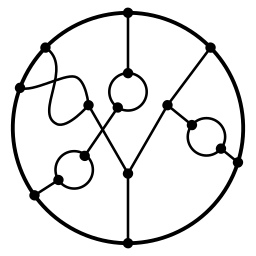
\includegraphics[width=0.13\textwidth, valign=c]{graphics/unitrivalent_diagram_example_2.pdf}
	\in \mathcal{T}.
\]

\begin{definition}
	An \textbf{STU relation} is a relation of the form
		\begin{equation}
			\label{eq:STU}
			\tag{\stu}
			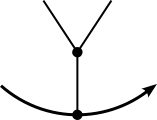
\includegraphics[width=0.10\textwidth, valign=c]{graphics/stu_relation_s.pdf}
			\quad
			=
			\quad
			\includegraphics[width=0.10\textwidth, valign=c]{graphics/stu_relation_t.pdf}
			\quad
			-
			\quad
			\includegraphics[width=0.10\textwidth, valign=c]{graphics/stu_relation_u.pdf}.
		\end{equation}
	Here the bottom line, drawn thicker and curved must be a part of the skeleton.
\end{definition}

As usual, this is not an individual relation but a class of relations, true in any diagrams that are identical except for the parts shown.

Note that the for the chord diagrams inside the algebra of Jacobi diagrams, the \ref{eq:STU} relations imply the \ref{eq:4T} relations, as
	\[
		\adjustbox{valign=c}{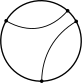
\includegraphics[width=0.115\textwidth]{graphics/four_term_from_stu_north.pdf}}
		\ - \
		\adjustbox{valign=c}{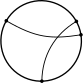
\includegraphics[width=0.115\textwidth]{graphics/four_term_from_stu_south.pdf}}
		\ = \
		\adjustbox{valign=c}{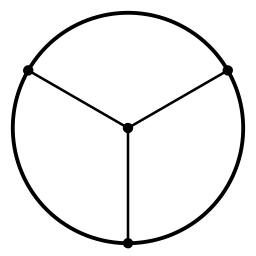
\includegraphics[width=0.12\textwidth]{four_term_jacobi_diagram.pdf}}
		\ = \
		\adjustbox{valign=c}{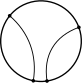
\includegraphics[width=0.115\textwidth]{graphics/four_term_from_stu_west.pdf}}
		\ - \
		\adjustbox{valign=c}{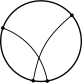
\includegraphics[width=0.115\textwidth]{graphics/four_term_from_stu_east.pdf}}\ .
	\]

\begin{definition}
	The algebra \(\mathcal{J}\) of Jacobi diagrams is the vector space \(\mathcal{T} / \ref{eq:STU}\), with the product \(\connect\) defined the same way as it was for chord diagrams.
\end{definition}

This is well-defined: the proof of Proposition \ref{prop:connected-sum-well-defined} showed that the product \(\connect\) being well-defined on \(\mathcal{A}\) was a consequence of the \ref{eq:4T} relations, which are implied by the \ref{eq:STU} relations. As such the \ref{eq:STU} relations suffice to determined the structure of \(\mathcal{J}\), but the following auxilliary relations which can be deduced from \ref{eq:STU} make the relations to Lie algebras more apparent.

\begin{proposition}
	\label{prop:stu-implies-as-ihx}
	The following relations are consequences of the \textup{\ref{eq:STU}} relation in \(\mathcal{J}\):
	\begin{enumerate}
		\item The \textbf{AS relation} (antisymmetry relation)
			\begin{equation}
				\label{eq:AS}
				\tag{\as}
				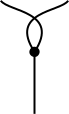
\includegraphics[width=0.05\textwidth, valign=c]{graphics/as_relation_a.pdf}
				\quad
				=
				\quad
				-
				\includegraphics[width=0.05\textwidth, valign=c]{graphics/as_relation_s.pdf}
			\end{equation}
		\item The \textbf{IHX relation}
			\begin{equation}
				\label{eq:IHX}
				\tag{\ihx}
				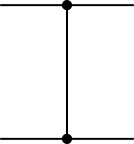
\includegraphics[width=0.10\textwidth, valign=c]{graphics/ihx_relation_i.pdf}
				\quad
				=
				\quad
				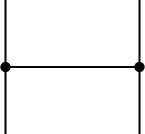
\includegraphics[width=0.10\textwidth, valign=c]{graphics/ihx_relation_h.pdf}
				\quad
				-
				\quad
				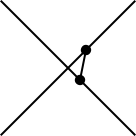
\includegraphics[width=0.10\textwidth, valign=c]{graphics/ihx_relation_x.pdf}
			\end{equation}
	\end{enumerate}
\end{proposition}

\begin{proof}
	\begin{enumerate}
		\item
			Take two diagrams which differ only by \ref{eq:AS} at one (trivalent) vertex. If the vertex at which the \ref{eq:AS} relation resides is adjacent to a univalent vertex (i.e. is adjacent to the skeleon), then this is immediate from applying \ref{eq:STU} to both diagrams at that vertex:
			\[
				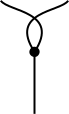
\includegraphics[width=0.05\textwidth, valign=c]{graphics/as_relation_a.pdf}
				\quad
				=
				\quad
				\includegraphics[width=0.10\textwidth, valign=c]{graphics/stu_relation_u.pdf}
				\quad
				-
				\quad
				\includegraphics[width=0.10\textwidth, valign=c]{graphics/stu_relation_t.pdf}
				\quad
				=
				\quad
				-
				\includegraphics[width=0.05\textwidth, valign=c]{graphics/as_relation_s.pdf}.
			\]
			If the vertex is not immediately adjacent to a univalent vertex, then it has some \(d\) trivalent vertices `in the way'. By applying \ref{eq:STU} to those vertices yields a sum of \(2^{d}\) diagrams, all identical except for differing by \ref{eq:AS}, now on a vertex adjacent to a univalent vertex.

		\item
			A similar argument applies. We give a sketch. If one of the two vertices of the \ref{eq:IHX} is adjacent to the skeleton, then the result is a direct consequence of an \ref{eq:STU} on each of the vertices in each of the diagrams in the \ref{eq:IHX}, followed by a few applications of \ref{eq:AS} (computing the twelve diagrams from applying two \ref{eq:STU}s to the three diagrams in an \ref{eq:IHX} verifies this; the computation is given in \cite[Lem. 5.2.6]{introduction-to-vassiliev-invariants}). Otherwise, there is a path of trivalent vertices in the way, and some \ref{eq:STU}s yield a sum of \(2^{d}\) diagrams in which at least one of the two vertices involved in the \ref{eq:IHX} is adjacent to the skeleton, and so the argument above applies.
\end{enumerate}
\end{proof}

\begin{proposition}[Generalised \ref{eq:IHX}]
	\label{lem:generalised-ihx}
	The following holds in \(\mathcal{J}\) for any subgraph consisting of trivalent vertices that can be inserted into the grey box.
	\[
		\sum_{i = 0}^{m}\
		\def\svgscale{0.3}
		\raisebox{-34pt}{\input{graphics/generalised_ihx_left.pdf_tex}}
		\quad
		=
		\quad
		\sum_{i = 0}^{n}\
		\def\svgscale{0.3}
		\raisebox{-34pt}{\input{graphics/generalised_ihx_right.pdf_tex}}
	\]
\end{proposition}

The result is standard --- see Chapter 5.2 of \cite{introduction-to-vassiliev-invariants} for a proof. A corollary is the following result, which will be important later.

\begin{proposition}
	\label{prop:linear-jacobi-diagrams-cyclically-invariant}
	If the univalent vertices of a Jacobi diagram are ordered linearly rather than cyclically, all linear orders that respect a given cyclic order are equivalent.
\end{proposition}

\begin{proof}
	Let us draw the linearly ordered Jacobi diagrams on a line rather than a circle and let the univalent edge ordering be given by the order on the line. It suffices to prove that we can move the univalent vertex in the first place to the last place via the relations in \(\mathcal{A}\). Let us call this first univalent vertex of the original diagram the marked vertex, as its position will later change when relations are applied. We will mark it with a star.

	By \ref{eq:STU}, the original diagram is equal to the diagram with the marked vertex moved into the second place, plus a diagram in which the marked vertex is now a trivalent vertex and attached above what was the second (but is now the first) univalent vertex:
	\[
		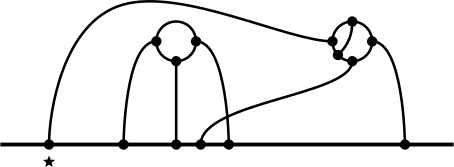
\includegraphics[width=0.25\textwidth, valign=c]{graphics/long_jacobi_diagram_example.pdf}
		\quad
		=
		\quad
		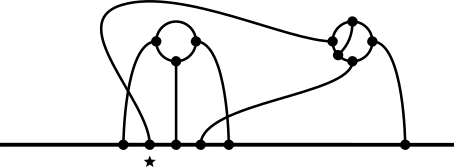
\includegraphics[width=0.25\textwidth, valign=c]{graphics/long_jacobi_diagram_example_t.pdf}
		\quad
		+
		\quad
		\includegraphics[width=0.25\textwidth, valign=c]{graphics/long_jacobi_diagram_example_u.pdf}
		.
	\]
	Repeatedly applying \ref{eq:STU} to move the the marked vertex until reaches the last place, we get
	\[
		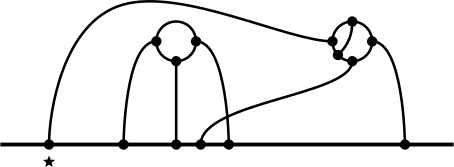
\includegraphics[width=0.25\textwidth, valign=c]{graphics/long_jacobi_diagram_example.pdf}
		\quad
		=
		\quad
		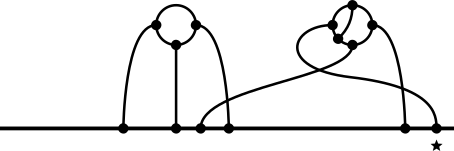
\includegraphics[width=0.25\textwidth, valign=c]{graphics/long_jacobi_diagram_example_final.pdf}
		\quad
		+
		\quad
		\Theta
	\]
	where \(\Theta\) is a sum of terms with the marked vertex now a trivalent vertex attached above each of the other univalent vertices. It suffices to show that \(\Theta\) vanishes.

	We can split \(\Theta\) up based on which connected component the marked vertex now connects to. For connected components other than the connected component of the marked vertex, apply a vertical version of the the generalised \ref{eq:IHX}, where the the whole connected component is inside the grey box except for where the univalent vertices connect to the bottom line. This is the case of the generalised \ref{eq:IHX} where \(n = 0\) and no vertices leave. Hence, the sum vanishes for that connected component.

	This leaves only the terms where the marked vertex connects back to its own connected component. By a generalised \ref{eq:IHX} of the form
	\[
		\sum \includegraphics[width=0.25\textwidth, valign=c]{graphics/long_jacobi_diagram_example_same_cc.pdf}\; ,
		\quad
		\text{this is equal to the diagram}
		\quad
		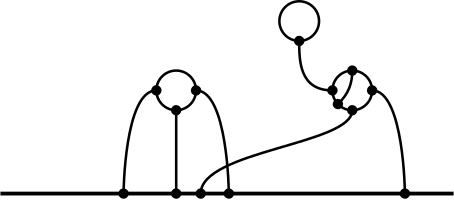
\includegraphics[width=0.25\textwidth, valign=c]{graphics/long_jacobi_diagram_example_lollipop.pdf}.
	\]
	But any diagram with a ``balloon'' vanishes, as applying the \ref{eq:AS} relation to the vertex on the balloon, it is equal to its negative.

	Hence \(\Theta = 0\), completing the proof.
\end{proof}

We have already spoiled the surprise that \(\mathcal{A}\) and \(\mathcal{J}\) are isomorphic as bialgebras. This is clearly true as \(\mathcal{J}\) is just a change of basis from \(\mathcal{A}\). Since \(\mathcal{A}\) spans \(\mathcal{J}\), we can attempt to lift the coproduct from \(\mathcal{A}\) directly onto \(\mathcal{J}\).

\begin{proposition}
	The coproduct \(\Delta\) on \(J \in \mathcal{J}\) defined by taking a Jacobi diagram, representing it as a chord diagram via \textup{\ref{eq:STU}}, taking the coproduct in \(\mathcal{A}\), then interpreting the result as a Jacobi diagram via the inclusion of \(\mathcal{A}\) into \(\mathcal{J}\) is given by the formula
	\[\Delta(J) = \sum_{C \subset S} J_{C} \otimes J_{\overline{C}}\]
	where \(S\) is the set of connected components of \(J\), and \(\overline{C} = S \smallsetminus C\).
\end{proposition}

\begin{proof}
	Note that this has the same symbolic form as the coproduct in \(\mathcal{A}\) given in Definition~\ref{def:coproduct-in-chord-diagrams}, but with chords replaced by connected components of Jacobi diagrams. However, when working in \(\mathcal{A} \subset \mathcal{J}\) there are only univalent vertices, so the connected components are exactly the chords. Since \(\mathcal{A}\) forms a basis for \(\mathcal{J}\) and the formula is linear, it extends to all of \(\mathcal{J}\).
\end{proof}

\begin{corollary}
	The primitive elements \(\mathcal{P}(\mathcal{A})\) are the connected Jacobi diagrams.
\end{corollary}

\begin{corollary}
	The bialgebras \(\mathcal{A}\) and \(\mathcal{J}\) are isomorphic.
\end{corollary}

\begin{warning}
	Justified by this isomorphism, we henceforth write \(\mathcal{A}\) for both chord diagrams and Jacobi diagrams.
\end{warning}

\section{Lie algebra weight systems}
Similar diagrammatic relations to \ref{eq:STU}, \ref{eq:AS} and \ref{eq:IHX} satisfied in \(\mathcal{A}\) appear also in the context of a graphical notation for multilinear maps, a fact which can be exploited to probe \(\mathcal{A}\). Before seeing how, let us review this graphical notation following \cite{wheeling-a-diagrammatic-analogue-of-the-duflo-isomorphism, on-the-rozansky-witten-weight-systems}. The diagrammatic calculus is well-known but it goes by many names: string diagram calculus, Penrose calculus, tensor calculus, diagrammatic calculus for tensors to name a few. We call them string diagrams.

A tensor is a multilinear map \(X_{1} \otimes X_{2} \otimes \cdots \otimes X_{n} \to Y_{1} \otimes Y_{2} \otimes \cdots \otimes Y_{m}\), or equivalently (via the canonical isomorphism) an element of the vector space \(X_{1}^{\ast} \otimes X_{2}^{\ast} \otimes \cdots X_{n}^{\ast} \otimes Y_{1} \otimes Y_{2} \otimes \cdots \otimes Y_{m}\). Such a tensor can be represented as a vertex with \(m + n\) unbound directed edges: \(m\) incoming edges decorated by the corresponding vector spaces (in the example above, \(X_{1}, \cdots X_{m}\)), and \(n\) outgoing edges decorated by \(Y_{1}, \cdots Y_{n}\). For example, the bracket in a Lie algebra \(\mathfrak{g}\) is an element \([\cdot,\cdot] \in \mathfrak{g}^{\ast} \otimes \mathfrak{g}^{\ast} \otimes \mathfrak{g}\) expressed as
\[\def\svgscale{0.3} \input{graphics/bracket_string_diagram.pdf_tex}.\]
It will be obvious from each string diagram what tensor it represents, so we drop the edge labels.

Such a notation is useful because composition of tensors can be expressed graphically by connecting outgoing and incoming legs with the same decoration. In particular relations can therefore be expressed graphically. For example, the antisymmetry of the bracket \({[y, x] = -[x, y]}\) becomes
\[
	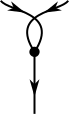
\includegraphics[width=0.05\textwidth, valign=c]{graphics/bracket_antisymmetry_swap.pdf}
	\quad
	=
	\quad
	-
	\includegraphics[width=0.05\textwidth, valign=c]{graphics/bracket_antisymmetry_id.pdf},
	\quad
	\text{and}
\]
the Jacobi relation \([[x, y], z] + [[y, z], x] + [[z, x], y] = 0\) becomes
\[
	\includegraphics[width=0.10\textwidth, valign=c]{graphics/jacobi_symmetric_xyz.pdf}
	\quad
	+
	\quad
	\includegraphics[width=0.10\textwidth, valign=c]{graphics/jacobi_symmetric_yzx.pdf}
	\quad
	+
	\quad
	\includegraphics[width=0.10\textwidth, valign=c]{graphics/jacobi_symmetric_zxy.pdf}
	\quad
	=
	\quad
	0
	.
\]

Looking at these relations in the tensor algebra \(\mathcal{T}(\mathfrak{g})\), a hint at the Lie-theoretic structure emerges. The antisymmetry of the bracket, (drawn as a string diagram) looks like a directed version of \ref{eq:AS}. Similarly the string diagrammmatic Jacobi relation can be arranged into a directed version of \ref{eq:IHX}.

Furthermore, suppose \(\mathfrak{g}\) is a metric Lie algebra so that it has an invariant, nondegenerate, bilinear form \(\langle \cdot, \cdot \rangle \in \mathfrak{g}^{\ast} \otimes \mathfrak{g}^{\ast}\). Being nondegenerate, it can be inverted to an element \(c \in \mathfrak{g} \otimes \mathfrak{g}\) --- this element is known as the Casimir element associated to \(\mathfrak{g}\) (or simply the Casimir). These tensors can be diagrammatically represented as additional bivalent vertices
\[
	\includegraphics[width=0.06\textwidth, valign=c]{graphics/string_diagram_metric.pdf}
	\qquad \text{and} \qquad
	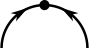
\includegraphics[width=0.06\textwidth, valign=c]{graphics/string_diagram_casimir.pdf}\ .
\]
Recall that the bilinear form induces an isomorphism of \(\mathfrak{g}\) and \(\mathfrak{g}^{\ast}\). Diagramatically, this can be used to change the arrow direction on any edge, allowing us to drop the edge arrows from the notation. Further, we also drop the dots in the metric and Casimir diagrams, so they look like
\[
	\includegraphics[width=0.06\textwidth, valign=c]{graphics/string_diagram_metric_no_dot.pdf}
	\qquad \text{and} \qquad
	\includegraphics[width=0.06\textwidth, valign=c]{graphics/string_diagram_casimir_no_dot.pdf}\ .
\]

Moreover, the invariance of the metric can be written as \(\langle [x, y], z \rangle = \langle [y, z], x \rangle\) which can be represented graphically as cyclic invariance of the contraction of the bracket and the metric:
\[
	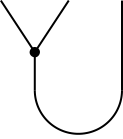
\includegraphics[width=0.08\textwidth, valign=c]{graphics/bracket_metric_cyclic_invariance_bracketxy.pdf}
	\quad
	=
	\quad
	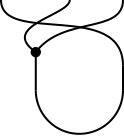
\includegraphics[width=0.08\textwidth, valign=c]{graphics/bracket_metric_cyclic_invariance_permute.pdf}
	\quad
	=
	\quad
	\includegraphics[width=0.08\textwidth, valign=c]{graphics/bracket_metric_cyclic_invariance_bracketyz.pdf}.
\]
A similar relation holds for the Casimir in a metric Lie algebra, namely if the Casimir is \({c = \sum_{i} e_{i} \otimes f_{i}}\), then for \(x \in \mathfrak{g}\), \(\sum_{i} e_{i} \otimes [f_{i}, x] = \sum_{i} [x, e_{i}] \otimes f_{i}\).
% NOTE: I actually don't know how to prove this only using properties of the metric (and therefore Casimir) and bracket.
Diagramatically, we have
\[
	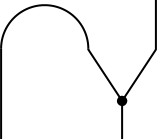
\includegraphics[width=0.1\textwidth, valign=c]{graphics/bracket_casimir_cyclic_invariance_left.pdf}
	\quad
	=
	\quad
	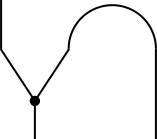
\includegraphics[width=0.1\textwidth, valign=c]{graphics/bracket_casimir_cyclic_invariance_right.pdf}
	\;
	.
\]
Just like the antisymmetry of the bracket and the Jacobi relation, these relations make sense when the diagrams are interpreted as parts of Jacobi diagrams. There is only one type of trivalent vertex in a Jaocbi diagram, and since the edges around a vertex are only considered up to cyclic order, cyclic permutation of the order is ``unseen on the level of Jacobi diagrams''.

From the discussion above, we see that the internal structure of Jacobi diagrams (internal meaning not near the skeleton) is reflected in a metric Lie algebra. Let us try to find a similar reflection of the structure near the skeleton. A representation \(\rho\) of \(\mathfrak{g}\) on a finite-dimensional vector space \(V\) can be written as a tensor \(\rho \in \mathfrak{g}^{\ast} \otimes V^{\ast} \otimes V\). This takes a new kind of input and output, namely a \(v \in V\) which we denote by a thicker line, like the skeleton of a Jacobi diagram.
\[
	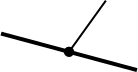
\includegraphics[width=0.11\textwidth, valign=c]{graphics/representation_vertex.pdf}
\]
We omit the arrows because they're unneccesary again --- corresponding to the maps
\[f \otimes v \longmapsto f(v) \quad \text{and} \quad 1 \longmapsto \sum_{i} e_{i} \otimes e_{i}^{\ast}\]
are vertices
\[
	\includegraphics[width=0.06\textwidth, valign=c]{graphics/string_diagram_eval.pdf}
	\qquad \text{and} \qquad
	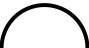
\includegraphics[width=0.06\textwidth, valign=c]{graphics/string_diagram_coeval.pdf}\ .
\]

That the action of \(\rho\) on \(V\) be a Lie action is the equation
\[\rho([x, y]) = \rho(x)\rho(y) - \rho(y)\rho(x)\]
which diagramatically corresponds to
\[
	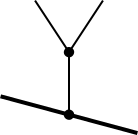
\includegraphics[width=0.1\textwidth, valign=c]{graphics/string_diagram_lie_action_s.pdf}
	\quad
	=
	\quad
	\includegraphics[width=0.1\textwidth, valign=c]{graphics/string_diagram_lie_action_t.pdf}
	\quad
	-
	\quad
	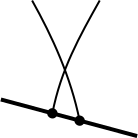
\includegraphics[width=0.1\textwidth, valign=c]{graphics/string_diagram_lie_action_u.pdf}.
\]

The following construction of Bar-Natan is the focus of his seminal article \cite{on-the-vassiliev-knot-invariants}. It uses this diagrammatic calculus to produce weight systems from metric Lie algebras.

\begin{construction}
	\label{cons:lie-algebra-weight-system}
	The construction takes a metric Lie algebra \(\mathfrak{g}\), and produces a map \({W_{\mathfrak{g}}: \mathcal{A} \to \mathcal{U}(\mathfrak{g})}\) which is a \(\mathcal{U}(\mathfrak{g})\)-valued weight system. Given further a representation \(\rho\) of \(\mathfrak{g}\) it produces a map \(W_{\mathfrak{g}}: \mathcal{A} \to k\) which is a \(k\)-valued weight system. That is, given \(\mathfrak{g}\) a metric Lie algebra and \(J \in \mathcal{A}\), it produces an element of \(\mathcal{U}(\mathfrak{g})\), and if also given a representation \(\rho\) it produces a scalar. We write \(v\) and \(u\) for the number of trivalent and univalent vertices respectively of \(J\).

	To each trivalent vertex of \(J\), associate a copy of the tensor \([\cdot, \cdot] \in \mathfrak{g}^{\ast} \otimes \mathfrak{g}^{\ast} \otimes \mathfrak{g}\) (see Warning \ref{warn:cyclic-order-of-bracket}). For each edge between trivalent vertices, contract the corresponding tensors along the components corresponding to those half-edges. Where the signature of the components doesn't allow for contraction (when both components are covariant or both are contravariant, i.e. when there are two inputs or two outputs), contract one of them first with either the metric or the casimir (whichever is allowed by its variance). The resulting tensor has \(u\) components (they may be co- or contra-variant).

	Contract this tensor with a copy of the casimir along all remaining covariant components. We define the result to be the tensor \(T_{\mathfrak{g}}(J) \in \mathfrak{g}^{\otimes u}\). The linear order of its components must be a linear order that agrees with the cyclic order of the corresponding univalent vertices in \(J\). Define \(W_{\mathfrak{g}}(J)\) to be the projection of this tensor into \(\mathcal{U}(\mathfrak{g})\), namely
	\[W_{\mathfrak{g}}(J) = [T_{\mathfrak{g}}(J)] \in \mathcal{U}(\mathfrak{g}).\]

	Constructing the \(k\)-valued weight system from the representation is as follows. A representation \(\rho: \mathfrak{g} \to \operatorname{Hom}(V)\) of a Lie algebra extends uniquely to a representation of its universal enveloping algebra \(\rho: \mathcal{U}(\mathfrak{g}) \to \operatorname{Hom}(V)\). Define \(W_{\mathfrak{g}, \rho}\) as the trace of \(W_{\mathfrak{g}}(J)\) with respect to this representation,
	\[W_{\mathfrak{g}, \rho}(J) = \operatorname{tr}(\rho(W_{\mathfrak{g}}(J))) \in \mathbb{Q}.\]
\end{construction}

\begin{warning}
	\label{warn:cyclic-order-of-bracket}
	In Construction \ref{cons:lie-algebra-weight-system} when constructing \(T_{\mathfrak{g}}(m)\), the tensor factors in the tensor corresponding to the bracket need to have the unusual cyclic order \((y^{\ast}, x^{\ast}, [x, y]_{\mathfrak{g}})\). This is because its projection into \(\mathcal{U}(\mathfrak{g})\) should obey \ref{eq:STU}, and this is the cyclic order of the trivalent vertex in \ref{eq:STU} (it will become evident in the proof why we need this convention).
\end{warning}

\begin{example}
	\label{ex:simple-sl2-computation}
	Take the metric Lie algebra \((\mathfrak{sl}_{2}, \langle \cdot, \cdot \rangle)\) where \(\mathfrak{sl}_{2}\) is defined by
	\[[h, e] = 2e, \quad [h, f] = -2f, \quad [e, f] = h,\]
	and the metric is
	\[\langle h, h \rangle = 2, \quad \langle e, f \rangle = 1, \quad \langle f, e \rangle = 1.\]
	Here we have chosen the normalisation of the metric that agrees with the trace in the adjoint representation, so
	\[
		[\cdot, \cdot]
		=
		2 e^{\ast} \otimes h^{\ast} \otimes e - 2 f^{\ast} \otimes h^{\ast} \otimes f + f^{\ast} \otimes e^{\ast} \otimes h.
	\]

	We do the computations for
	\[	
		J = 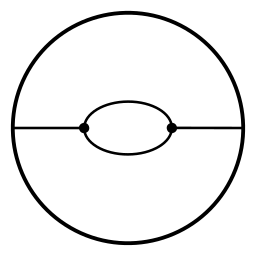
\includegraphics[width=0.1\textwidth, valign=c]{graphics/jacobi_bivalent_bubble.pdf}.
	\]
	Taking another copy \([\cdot, \cdot]'\) of the bracket tensor, one way to compute \(W_{\mathfrak{sl}_{2}} \left( J \right)\) is to let \([\cdot,\cdot]\) take the left trivalent vertex, and associate the upward facing half-edge to the first component. Let \([\cdot,\cdot]'\) take the right trivalent vertex and associate the downward facing half-edge to the first component --- the cyclic orders determine the rest. Then the computation is to take the contraction of \([\cdot,\cdot]\) along components 1 and 3 with \([\cdot,\cdot]'\) along components 3 and 1. This gives
	\[2 h^{\ast} \otimes h^{\ast} + e^{\ast} \otimes f^{\ast} + f^{\ast} \otimes e^{\ast},\]
	and contracting along each component with a casimir to make them contravariant yields
	\[
		T_{\mathfrak{sl}_{2}}
		\left(
		J
		\right)
		=
		\frac{1}{2} h \otimes h + e \otimes f + f \otimes e.
	\]
	Projecting this into \(\mathcal{U}(\mathfrak{g})\) and writing it in the PBW-basis, we have
	\[W_{\mathfrak{sl}_{2}}(J) = \frac{1}{2} h \otimes h - h + 2 e \otimes f.\]

	Finally, if we use the adjoint representation \(\operatorname{ad}\), defined by
	\[
		\operatorname{ad}(h) =
		\begin{bmatrix}
			1 & 0 \\
			0 & -1
		\end{bmatrix}\;,\quad
		\operatorname{ad}(e) =
		\begin{bmatrix}
			0 & 1 \\
			0 & 0
		\end{bmatrix}\;,\quad
		\operatorname{ad}(f) =
		\begin{bmatrix}
			0 & 0 \\
			1 & 0
		\end{bmatrix}\;,\quad
	\]
	we get
	\[W_{\mathfrak{sl}_{2}, \operatorname{ad}}(J) = 3.\]
\end{example}

\begin{theorem}
	In Construction \ref{cons:lie-algebra-weight-system}, \(W_{\mathfrak{g}}\) is a well-defined \(\mathcal{U}(\mathfrak{g})\)-valued weight system, and \(W_{\mathfrak{g}, \rho}\) is a well-defined \(k\)-valued weight system.
\end{theorem}

\begin{proof}[\cite{on-the-vassiliev-knot-invariants}]
	First we prove that the map \(W_{\mathfrak{g}}: \mathcal{D} \to \mathcal{U}(\mathfrak{g})\) descends to a map from \(\mathcal{A}\).

	The map \(T_{\mathfrak{g}}: \mathcal{D} \to \mathfrak{g}^{\otimes u}\) is invariant under \ref{eq:IHX} and \ref{eq:AS}: for \ref{eq:AS}, it follows from the antisymmetry of \([\cdot, \cdot]\), and for \ref{eq:IHX} it follows from the Jacobi relation.

	Furthermore, the map \(\mathfrak{g}^{\otimes u} \to \mathcal{U}(\mathfrak{g})\) is invariant under \ref{eq:STU}. For if two chord diagrams differ by \ref{eq:STU}, on some univalent vertices associated with adjacent tensor factors \(y\) and \(x\), the two sides of an \ref{eq:STU} map to
	\[\cdots \otimes [x, y]_{\mathfrak{g}} \otimes \cdots \qquad \text{and} \qquad (\cdots \otimes x \otimes y \otimes \cdots) - (\cdots \otimes y \otimes x \otimes \cdots),\]
	but the equality of these expressions is exactly the defining relation of \(\mathcal{U}(\mathfrak{g})\). (Alternatively the well-definiedness of \(W_{\mathfrak{g}}\) under \ref{eq:AS} and \ref{eq:IHX} also follows from this, because those relations are implied by \ref{eq:STU}.)

	There is one other arbitrary choice that was made in the construction. The cyclic order of the univalent vertices of \(J\) induces a cyclic order on the components of the components of the tensor \(T_{\mathfrak{g}} \in \mathfrak{g}^{\otimes u}\). However, in the construction, a linear order which respects that cyclic order was chosen. We must show that any choice of linear order respecting the cyclic order produces the same result. This is no problem for the well-definedness of \(W_{\mathfrak{g}, \rho}(J) = \operatorname{tr}(\rho(W_{\mathfrak{g}}(J)))\), as the trace is invariant under cyclic permutation. However for \(W_{\mathfrak{g}}(J) = [T_{\mathfrak{g}}(J)] \in \mathcal{U}(\mathfrak{g})\) it remains to prove cyclic permutation invariance. In fact, a stronger statement is true. The diagram \(J\) itself is invariant under a cyclic permutation by Proposition \ref{prop:linear-jacobi-diagrams-cyclically-invariant}, so of course this is true for \(W_{\mathfrak{g}}(J)\).
\end{proof}

Let's look at a specific weight system for the Lie algebra \(\mathfrak{sl}_{2}\) \cite{on-the-vassiliev-knot-invariants, remarks-on-the-vassiliev-knot-invariants-coming-from-sl2}.
\begin{example}[Weight system for \({\mathfrak{sl}_{2}}\)]
	\label{ex:sl2-cv-relation}
	We use the metric Lie algebra from Example \ref{ex:simple-sl2-computation}. In \cite{remarks-on-the-vassiliev-knot-invariants-coming-from-sl2}, the following skein relation is derived:
	% NOTE: We are using the trace in the fundamental representation as our invariant bilinear form. If instead, we used the trace in the adjoint representation, we would get coefficients 1 instead of 4.
	\[
		W_{\mathfrak{sl}_{2}}
			\includegraphics[width=0.115\textwidth, valign=c]{graphics/sl2_skein_relation_h.pdf}
		=
		2 W_{\mathfrak{sl}_{2}}
			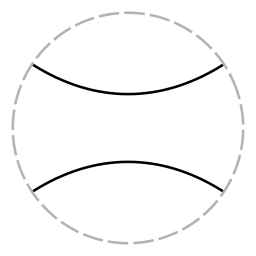
\includegraphics[width=0.115\textwidth, valign=c]{graphics/sl2_skein_relation_uu.pdf}
		-
		2 W_{\mathfrak{sl}_{2}}
			\includegraphics[width=0.115\textwidth, valign=c]{graphics/sl2_skein_relation_x.pdf}
	\]
\end{example}

	\begin{proof}
		Compute both sides like in Construction \ref{cons:lie-algebra-weight-system}, but without projecting into \(\mathcal{U}(\mathfrak{g})\), leaving the result in \(\mathfrak{sl}_{2}^{\otimes 4}\). Both give
		\begin{align*}
			{}-h\otimes e\otimes h\otimes f+h\otimes e\otimes f\otimes h-h\otimes f\otimes h\otimes e+h\otimes f\otimes e\otimes h \\
			{}+e\otimes h\otimes h\otimes f-e\otimes h\otimes f\otimes h + 2 e\otimes f\otimes e\otimes f -2 e\otimes f\otimes f\otimes e \\
			{}+f\otimes h\otimes h\otimes e -f\otimes h\otimes e\otimes h -2 f\otimes e\otimes e\otimes f + 2 f\otimes e\otimes f\otimes e.
		\end{align*}
	\end{proof}

	\begin{remark}
		\label{rem:metric-casimir-bubble-is-dimension}
		When computing via the \(\mathfrak{sl}_{2}\) skein relation above, it's possible to create a ``bubble'' (part of a diagram without any trivalent vertices). Since we are computing via contractions in the tensor algebra, this is to be interpreted as the contraction of the metric with the casimir. In a finite-dimensional Lie algebra, this is just the dimension (so for \(\mathfrak{sl}_{2}\), the factor \(3\)). For example,
		\[
			W_{\mathfrak{sl}_{2}}
			\includegraphics[width=0.115\textwidth, valign=c]{graphics/jacobi_diagram_with_bubble.pdf}
			\quad
			=
			\quad
			3 W_{\mathfrak{sl}_{2}}
			\includegraphics[width=0.115\textwidth, valign=c]{graphics/jacobi_diagram_with_bubble_removed.pdf}.
		\]
	\end{remark}
\begin{question}
	In \cite[Remark 16.9]{introduction-to-vassiliev-invariants} it is noted that the \(\mathfrak{sl}_{2}\) skein relation is an analogue of the vector triple product rule for the cross product in \(\mathbb{R}^{3}\). The relation has been further studied in \cite{riordan-trees-and-the-homotopy-sl2-weight-system} to determine a basis for \(\mathcal{W}_{\mathfrak{sl}_{2}}\). There is also a cross product in \(\mathbb{R}^{7}\), related to the exceptional Lie algebra \(\mathfrak{g}_{2}\) --- it also obeys a variant of the vector triple product rule. Is there a similar skein relation for \(\mathcal{W}_{\mathfrak{g}_{2}}\)? Are there other skein relations that the weight systems for the exceptional Lie algebras obey?
\end{question}

Construction \ref{cons:lie-algebra-weight-system} yields a way of extracting some information from \(\mathcal{A}\) by plugging in a metric Lie algebra -- doing so constructs some quotient of \(\mathcal{A}\). This leads to the natural question of whether all of the information in \(\mathcal{A}\) can be extracted by metric Lie algebras in the manner of the construction.

A computer enumeration of \cite{on-the-vassiliev-knot-invariants} proves this for order \(m \leq 9\):
\[
	\begin{tblr}{hlines, vlines, colspec={lcccccccccc}}
		m									& 0 & 1 & 2 & 3 & 4 & 5  & 6  & 7  & 8  & 9   \\ % & 10  & 11  & 12  \\
		\operatorname{dim} \mathcal{W}_{m}					& 1 & 1 & 2 & 3 & 6 & 10 & 19 & 33 & 60 & 104 \\ % & 184 & 316 & 548 \\
		\operatorname{dim} (\mathcal{W}_{\text{Lie}})_{m}			& 1 & 1 & 2 & 3 & 6 & 10 & 19 & 33 & 60 & 104 \\
	\end{tblr}
\]
(here \(\mathcal{W}_{\text{Lie}}\) denotes the dimension of the subspace of \(\mathcal{W}_{m}\) spanned by weight systems coming from Construction \ref{cons:lie-algebra-weight-system}). In other words
\[\mathcal{W}_{\text{Lie}} = \operatorname{span} \{W_{\mathfrak{g}, \rho} \,|\, \text{\(\mathfrak{g}\) a Lie algebra}, \text{\(\rho\) a representation of \(\mathfrak{g}\)}\}.\]
In \cite{on-the-vassiliev-knot-invariants}, this is computed up to degree \(9\) only using the span of \(\mathfrak{sl}_{n}\) and \(\mathfrak{gl}_{n}\) Lie algebras, providing a lower bound on \(\operatorname{dim} (\mathcal{W}_{\text{Lie}})_{m}\). The upper bound comes from \(\operatorname{dim} \mathcal{A}_{m}\). So in fact, up to degree \(9\), \(\mathcal{W}_{m}\) is spanned even by only the \(\mathfrak{sl}_{n}\) and \(\mathfrak{gl}_{n}\) weight systems.

\begin{conjecture}[Bar-Natan]
	\label{conj:lie-algebra-weight-systems-span}
	All weight systems are obtained as Lie algebra weight systems. In other words, the set \(\{W_{\mathfrak{g}, \rho} \,|\, \text{\(\mathfrak{g}\) a Lie algebra}, \text{\(\rho\) a representation of \(\mathfrak{g}\)}\}\) spans \(\mathcal{W}\).
\end{conjecture}

Indeed, the Lie action relation \(\rho([x, y]) = \rho(x)\rho(y) - \rho(y)\rho(x)\) as it was drawn graphically looks exactly like the \ref{eq:STU} relation in \(\mathcal{A}\). However, looks turn out to be decieving and quite surprisingly this conjecture is false. The counterexample was found by Pierre Vogel \cite{algebraic-structures-on-modules-of-diagrams-preprint} in an attempt to answer the following related question:
\begin{question}[Vogel]
	\label{ques:vogel-universal-lie-algebra}
	Is there some single universal Lie algebra object whose weight system spans \(W_{\text{Lie}}\), the span of all Lie-algebraic weight systems?
\end{question}

\section{Non-Lie algebraic weight systems}
\label{sec:non-lie-algebraic-weight-systems}

Conjecture \ref{conj:lie-algebra-weight-systems-span} being false means that the \ref{eq:STU} relation describes more than the relation \(\rho([x, y]) = \rho(x)\rho(y) - \rho(y)\rho(x)\) for a representation \(\rho\) of a metric Lie algebra. In fact, Construction \ref{cons:lie-algebra-weight-system} is just one example of a more general construction introduced by Vogel and Vaintrob with the purpose of constructing weight systems coming from metric Lie super-algebras, and further generalisations of Lie algebras.

The most general type of objects these constructions apply to are `Lie \(S\)-algebras' as coined by Vaintrob in \cite{vassiliev-knot-invariants-and-lie-s-algebras}, but we will follow the more modern approach of \cite{on-the-rozansky-witten-weight-systems, rozansky-witten-theory} and will refer to them as Lie algebra objects in a symmetric monoidal category.

\begin{definition}
	A (\textbf{weak}) \textbf{monoidal category} is a category \(\mathcal{C}\) equipped with a functor
	\[
		\begin{array}{rccc}
			\otimes:	&\mathcal{C} \times \mathcal{C}		&\longrightarrow	&\mathcal{C}\\
					&(A, B)					&\longmapsto		&A \otimes B,
		\end{array}
	\]
	a \textbf{unit} object \(k \in \mathcal{C}\), and natural isomorphisms
	\[
		 \otimes \circ (\otimes \times \operatorname{id}) \longrightarrow \otimes \circ (\operatorname{id} \times \otimes)  \quad \text{ and }\ \quad  \otimes \longrightarrow \operatorname{id}
	\]
	satisfying some relations known as the pentagon and triangle relations \cite[Sec. 1.2]{higher-operads-higher-categories}. The natural isomorphisms give isomorphisms
	\[(A \otimes B) \otimes C \cong A \otimes (B \otimes C), \qquad k \otimes A \cong A \cong A \otimes k\]
	for every tuple of objects \(A, B\) and \(C\) in \(\mathcal{C}\). If these isomorphisms are equalities, then \(\mathcal{C}\) is a \textbf{strict} monoidal category.
\end{definition}

\begin{remark}
	\label{rem:coherence-for-monoidal-categories}
	While we omit the details, we henceforth assume that these natural isomorphisms are equalities: \((A \otimes B) \otimes C = A \otimes (B \otimes C)\). This is acceptable by the coherence theorem for monoidal categories which says that every monoidal category is equivalent to a strict monoidal category. This also justifies why we omit the pentagon and triangle relations in the definition above. We refer the reader to \cite[Sec. 1.2]{higher-operads-higher-categories} for details.
\end{remark}

\begin{definitions}
	\begin{enumerate}
		\item The \textbf{flip functor} is the functor
			\[
				\begin{array}{rccc}
					\sigma:		&\mathcal{C} \times \mathcal{C}		&\longrightarrow	&\mathcal{C} \times \mathcal{C}\\
						&(A, B)					&\longmapsto		&(B, A).
				\end{array}
			\]

		\item A \textbf{symmetric monoidal category} is a monoidal category \(\mathcal{C}\) equipped with a \textbf{symmetry natural isomorphism}
			\[\tau : \otimes \longrightarrow \otimes \circ \sigma\]
			satisfying the hexagon relation. The \textbf{hexagon relation} is the relation that the isomorphisms
			\[
				\tau_{A, B}: A \otimes B \overset{\cong}{\longrightarrow} B \otimes A
			\]
			and
			coming from the natural isomorphism \(\tau\) obey
			\[\tau_{A, B \otimes C} = (\operatorname{id}_{B} \mathbin{\otimes} \tau_{A, C}) \circ (\tau_{A, B} \mathbin{\otimes} \operatorname{id}_{C})\]
			for every pair of objects \(A\), and \(B\) in \(\mathcal{C}\). 
	\end{enumerate}
\end{definitions}
One might notice that the hexagon relation involves only three terms, rather than the six that the name might suggest. This is because we have omited the reassociation natural isomorphisms that we can assume are identities by Remark \ref{rem:coherence-for-monoidal-categories}.

If a monoidal category \(\mathcal{C}\) is additionally additive, we can define Lie algebra objects internal to \(\mathcal{C}\).

\begin{definitions}
	\label{def:internal-to-additive-monoidal-category}
	\begin{enumerate}
		\item A \textbf{Lie algebra object} in an additive symmetric tensor category \(\mathcal{C}\) is an object \(L\) equipped with a bracket morphism \(\beta : \mathcal{C} \otimes \mathcal{C} \to \mathcal{C}\) such that
			\[\left( \beta \circ (\beta \otimes \operatorname{id}) \right) \circ (1 + \tau_{123} + (\tau_{123})^{2}) = 0 \qquad \text{and} \qquad \beta + \beta \circ \tau = 0.\]
			Graphically (in terms of the string diagrams of the previous section), this corresponds to
			\[
				\def\svgscale{0.31}
				\adjustbox{valign=c}{\input{graphics/jacobi_symmetric_arbitrary_monoidal_cat_xyz.pdf_tex}}
				\quad
				+
				\quad
				\def\svgscale{0.31}
				\adjustbox{valign=c}{\input{graphics/jacobi_symmetric_arbitrary_monoidal_cat_yzx.pdf_tex}}
				\quad
				+
				\quad
				\def\svgscale{0.31}
				\adjustbox{valign=c}{\input{graphics/jacobi_symmetric_arbitrary_monoidal_cat_zxy.pdf_tex}}
				\quad
				=
				\quad
				0,
				\quad
				\text{and}
			\]
			\[
				\def\svgscale{0.35}
				\adjustbox{valign=c}{\input{graphics/bracket_antisymmetry_arb_mon_cat_id.pdf_tex}}
				\quad
				+
				\quad
				\def\svgscale{0.35}
				\adjustbox{valign=c}{\input{graphics/bracket_antisymmetry_arb_mon_cat_swap.pdf_tex}}
				\quad
				=
				\quad
				0.
			\]
			Here the trivalent vertex corresponds to the \(\beta\) the generalised bracket morphism.
		\item A (right) \textbf{module \(\rho\) over a Lie algebra object \(L\) in \(\mathcal{C}\)} is an object \(M\) with a morphism \(\rho: M \otimes L \to M\), diagramatically denoted
			\[
				\includegraphics[width=0.11\textwidth, valign=c]{graphics/representation_vertex_before_dualisable.pdf}
			\]
			such that
			\[\rho \circ (\id \otimes \beta) = \rho \circ (\rho \otimes \id ) \circ (\id \otimes \tau).\]
			Here the thick line denotes \(M\) and this type of trivalent vertex denotes \(\rho\). As a string diagram this becomes
			\[
				\def\svgscale{0.31}
				\adjustbox{valign=c}{\input{graphics/string_diagram_lie_action_arb_mon_cat_s.pdf_tex}}
				\quad
				=
				\quad
				\def\svgscale{0.31}
				\adjustbox{valign=c}{\input{graphics/string_diagram_lie_action_arb_mon_cat_t.pdf_tex}}
				\quad
				-
				\quad
				\def\svgscale{0.31}
				\adjustbox{valign=c}{\input{graphics/string_diagram_lie_action_arb_mon_cat_u.pdf_tex}}
				.
			\]

			Note that any right module \(M\) can be given a natural left-module structure by
			\[\bar{\rho} = - \rho \circ \tau\]
			justifying the diagrammatic rule
			\[
				\includegraphics[width=0.11\textwidth, valign=c]{graphics/representation_vertex_before_dualisable.pdf}
				\quad
				=
				\quad
				-
				\includegraphics[width=0.11\textwidth, valign=c]{graphics/representation_vertex_before_dualisable_flipped.pdf}
				\;
				.
			\]

		\item A \textbf{metric Lie algebra object} \(L\) in \(\mathcal{C}\) is a Lie algebra object in \(\mathcal{C}\), further equipped with a metric morphism \(m: L \otimes L \to k\) and Casimir morphism \(c: k \to L \otimes L\) which abstract the metric and Casimir of Lie algebras in \(\mathbf{Vect}\) by satisfying
			\[(\id \otimes c) \circ (m \otimes \id) = \id = (c \otimes \id) \circ (\id \otimes m)\]
			and
			\[m = \tau \circ m \quad \text{and} \quad c = c \circ \tau.\]
			Diagramatically, these are
			\[
				\includegraphics[width=0.06\textwidth, valign=c]{graphics/string_diagram_metric_no_dot.pdf}
				\qquad \text{and} \qquad
				\includegraphics[width=0.06\textwidth, valign=c]{graphics/string_diagram_casimir_no_dot.pdf}\ .
			\]
			(like before these morphisms allow us to drop arrows on the thin lines) satisfying
			\[
				\includegraphics[height=0.12\textwidth, valign=c]{graphics/string_diagram_relation_left.pdf}
				\quad
				=
				\quad
				\includegraphics[height=0.12\textwidth, valign=c]{graphics/string_diagram_relation_middle.pdf}
				\quad
				=
				\quad
				\includegraphics[height=0.12\textwidth, valign=c]{graphics/string_diagram_relation_right.pdf}
				\quad
			\]
			and the second and third relations assert that the diagrams are symmetric.
		\item
			\label{def:rigid-category-and-object}
			A monoidal category \(\mathcal{C}\) is \textbf{rigid} if for every object \(A\) there exists an object \(A^{\vee}\) and a pair of morphisms \(\iota: A^{\vee} \otimes A \to k\) and \(\epsilon: k \to A \otimes A^{\vee}\) --- respectively called the \textbf{evaluation} and \textbf{coevaluation} --- such that
			\[(\id_{A} \otimes \epsilon) \circ (\iota \otimes \id_{A}) = \id_{A}\]
			and
			\[(\epsilon \otimes \id_{A^{\vee}}) \circ (\id_{A^{\vee}} \otimes \iota) = \id_{A^{\vee}}\]
			Diagramatically, these are
			\[
				\includegraphics[height=0.12\textwidth, valign=c]{graphics/string_diagram_rigidity_snake.pdf}
				\quad
				=
				\quad
				\includegraphics[height=0.12\textwidth, valign=c]{graphics/string_diagram_rigidity_id.pdf}
				\qquad
				\text{and}
				\qquad
				\includegraphics[height=0.12\textwidth, valign=c]{graphics/string_diagram_rigidity_dual_snake.pdf}
				\quad
				=
				\quad
				\includegraphics[height=0.12\textwidth, valign=c]{graphics/string_diagram_rigidity_dual_id.pdf}
				\;.
			\]
			
			An object in a monoidal category \(\mathcal{C}\) is \textbf{rigid} if axioms above are satisfied just for that object without the whole category needing to be rigid.
	\end{enumerate}
\end{definitions}

For a rigid monoidal category \(\mathcal{C}\), the dual of a (right) module may be turned into a (right) module by asserting that the module action commutes with the evaluation and coevaluation (that is evaluation and coevaluation are module maps). Diagramatically,
\[
	\includegraphics[height=0.12\textwidth, valign=c]{graphics/string_diagram_module_dual.pdf}
	\quad
	=
	\quad
	-
	\quad
	\includegraphics[height=0.12\textwidth, valign=c]{graphics/string_diagram_eval_coeval_module_maps.pdf}
	.
\]
\begin{shaded}
	Question: How do I explain the minus sign here? I imagine it's to do wth the minus sign in left/right module statement above.
\end{shaded}

We will give various concrete examples of Lie algebra objects in different symmetric monoidal categories later. For now, let's show that this data can be used to construct weight systems, generalising Construction \ref{cons:lie-algebra-weight-system}.

\begin{theorem}[\cite{vassiliev-knot-invariants-and-lie-s-algebras}]
	Let \(\mathcal{C}\) be a rigid, additive, symmetric monoidal category, \(L\) a metric Lie algebra in \(\mathcal{C}\), and \(M\) a rigid module (a rigid object in the monoidal category of modules over \(L\)).
	Then there is a weight system
	\[W_{L, M}: \mathcal{A} \longrightarrow \mathcal{C}(k, k).\]
	If \(\mathcal{C}\) is \(k\)-linear, then this is a \(k\)-valued weight system
	\[W_{L, M}: \mathcal{A} \longrightarrow k.\]
\end{theorem}

The proof of this theorem is exactly the same as the proof of construction \ref{cons:lie-algebra-weight-system}, but considering everything in the generality of \(\mathcal{C}\) rather than \(\mathbf{Vect}\). It is proved in \cite{on-the-rozansky-witten-weight-systems}.

The difference between this construction and Construction \ref{cons:lie-algebra-weight-system} is the treatment of the symmetry natural isomorphism \(\tau\) which tells us what isomorphism to use when rearranging the tensor factors. The most obvious isomorphism would be the identity (as it was in the original construction) corresponding to when \(\mathcal{C}\) is a strict symmetric (strict) monoidal category. However not every symmetric monoidal category is equivalent to a strict symmetric monoidal category. In other words, Lie algebra objects with non-trivial symmetry isomorphisms are necessary to pick up all the structure in \(\mathcal{A}\).

\begin{example}
	If we take \(\mathcal{C} = \mathbf{sVect}\), the symmetric monoidal category of super vector spaces, the Lie algebra objects are exactly the Lie superalgebras which we now define.

	A \textbf{Lie superalgebra} \(\mathfrak{g}\) is a vector space with a \(\mathbb{Z} / 2\mathbb{Z}\) grading, equipped with a bracket \([\cdot,\cdot]: \mathfrak{g} \otimes \mathfrak{g} \to \mathfrak{g}\) satisfying two axions. The \textbf{super symmetry} axiom is that for \(x, y\) homogeneous elements of \(\mathfrak{g}_{i}\) and \(\mathfrak{g}_{j}\) respectively,
	\[[x, y] = - (-1)^{ij}[y, x]\]
	and the \textbf{super Jacobi identity}, that for homogeneous elements \(x, y\) and \(z\) in \(\mathfrak{g}_{i}, \mathfrak{g}_{j}\) and \(\mathfrak{g}_{k}\),
	\[(-1)^{ik}[x, [y, z]] + (-1)^{ji}[y, [z, x]] + (-1)^{kj}[z, [x, y]] = 0.\]

	The grading induces the splitting \(\mathfrak{g} = \mathfrak{g}_{0} \oplus \mathfrak{g}_{1}\), and the direct summand \(\mathfrak{g}_{0}\) is known as the \textbf{even} part and the summand \(\mathfrak{g}_{1}\) is known as the \textbf{odd} part.
\end{example}

Shortly after Conjecture \ref{conj:lie-algebra-weight-systems-span} was made, the following results were achieved based on constructions with the exceptional Lie superalgebra \(\mathfrak{D}(2, 1; \alpha)\) proving that metric Lie algebras alone do not see all the structure of \(\mathcal{A}\).

\begin{theorem}
	There are primitive Jacobi diagrams of order 17 \cite{algebraic-structures-on-modules-of-diagrams-preprint} and 15 \cite{on-vassiliev-invariants-not-coming-from-semisimple-lie-algebras} which vanish under all Lie algebra weight systems.
\end{theorem}

Indeed (and this was known about shortly after but not published until significantly later) not even metric Lie superalgebras suffice.

\begin{theorem}
	Vogel's diagram of order 17 vanishes also on all Lie superalgebra weight systems \cite{algebraic-structures-on-modules-of-diagrams}.
\end{theorem}

\begin{corollary}
	The set of Lie (super)algebra weight systems does not span \(\mathcal{W}\).
\end{corollary}

In general, it is still unknown what exact level of generality one needs (what type of symmetric monoidal categories need to be considered) in order to generate all weight systems. We hereby provide a succinct review of the current state of the literature on the subject.

Roberts and Willerton in \cite{rozansky-witten-theory} and \cite{on-the-rozansky-witten-weight-systems} examine weight systems constructructed from Lie algebra objects in the derived category of complex manifolds. Such weight systems are candidates for being able to detect knot orientation, which Lie algebra weight systems cannot \cite{on-the-vassiliev-knot-invariants}. However, computing these weight systems is difficult, and to our knowledge, no computations exist in the literature.

More recently Aizawa-Kimura \cite{universal-weight-systems-from-a-mimimal-Z22-graded-lie-algebra} have conducted some preliminary investigations into the class of colour Lie algebras (also known as \(\epsilon\)-Lie algebras). This class generalises the \(\mathbb{Z}/2\mathbb{Z}\) grading on Lie superalgebras to a more general group. However, the example they present lies within the span of the \(\mathfrak{sl}_{2}\) and \(\mathfrak{gl}_{1 | 1}\) weight systems.


\section{Some weight systems at the exceptional Lie algebras}
\label{sec:some-weight-systems-at-the-exceptional-lie-algebras}

The original motivation for the work of Vogel \cite{algebraic-structures-on-modules-of-diagrams-preprint, algebraic-structures-on-modules-of-diagrams} (seen more explicity in \cite{vassiliev-theory-and-the-universal-lie-algebra}) was to construct a universal object generalising all simple Lie algebras. Such an object would parametrise the relations in tensor powers of the adjoint representation of all simple Lie algebras, and its weight systems would span \(\mathcal{W}\). For example, the relation for \(W_{\mathfrak{sl}_{2}}\) given in Example \ref{ex:sl2-cv-relation} is entirely internal to the Lie algebra; it doesn't involve projecting to the universal enveloping algebra or choosing a representation (since the adjoint representation is canonical).

Recently, it seems there is renewed interest in Vogel's methods \cite{construction-of-lie-algebra-weight-system-kernel-via-vogel-algebra, on-refined-vogels-universality, can-yang-baxter-imply-lie-algebra}. In-particular, present implicitly in \cite{algebraic-structures-on-modules-of-diagrams} is a way to determine local relations internal to any simple Lie algebra in terms of two independent ``Vogel parameters'', and some complicated marked elements of \(\mathcal{A}\) defined recursively. These were written out explicitly in \cite[Appendix]{construction-of-lie-algebra-weight-system-kernel-via-vogel-algebra}, but the use of different normalisations of the Vogel parameters between this and \cite{algebraic-structures-on-modules-of-diagrams} makes computing explicit relations tedious. Moreover, the relations in Vogel's original work, are general enough to hold for any Lie superalgebra but when restricting to Lie algebras, the diagrammatic formulae can be simplified.

For example, \cite[Theorem 6.3(2)]{algebraic-structures-on-modules-of-diagrams} gives the relation
\[
	\begin{array}{ll}
		-6
		W_{\mathfrak{g}_{2}}
		\includegraphics[width=0.115\textwidth, valign=c]{graphics/local_jacobi_w4_column.pdf}
		-
		12
		W_{\mathfrak{g}_{2}}
		\includegraphics[width=0.115\textwidth, valign=c]{graphics/local_jacobi_w4_crossbeam.pdf}
		+
		18
		W_{\mathfrak{g}_{2}}
		\includegraphics[width=0.115\textwidth, valign=c]{graphics/local_jacobi_tw4.pdf} \\
		\quad
		{}+\displaystyle\frac{7}{4}
		W_{\mathfrak{g}_{2}}
		\includegraphics[width=0.115\textwidth, valign=c]{graphics/local_jacobi_tth.pdf}
		+
		20
		W_{\mathfrak{g}_{2}}
		\includegraphics[width=0.115\textwidth, valign=c]{graphics/local_jacobi_smooth.pdf}
		+
		20
		W_{\mathfrak{g}_{2}}
		\includegraphics[width=0.115\textwidth, valign=c]{graphics/local_jacobi_cross.pdf}
		& =
		\,\,\,
		0
	\end{array}
\]
in \(\mathcal{W}_{\mathfrak{g}_{2}}\). By some well-known identites internal to Jacobi diagrams, this relation can be simplified.
\begin{lemma}
	\label{lem:tribubble-is-half-bibubble}
	In \(\mathcal{A}\), the `trivalent-bubble' vertex is proportional to the regular trivalent vertex with a bivalent bubble inserted on any one of the half-edges.
	\[
		\includegraphics[width=0.115\textwidth, valign=c]{graphics/local_jacobi_triangle.pdf}
		=
		\frac{1}{2}
		\includegraphics[width=0.115\textwidth, valign=c]{graphics/local_jacobi_triangle_bubbled.pdf}
	\]
\end{lemma}
\begin{proof}
	Apply \ref{eq:IHX} to any pair of vertices, followed by three applications of \ref{eq:AS}.
	\[
		\includegraphics[width=0.115\textwidth, valign=c]{graphics/local_jacobi_triangle.pdf}
		=
		\includegraphics[width=0.115\textwidth, valign=c]{graphics/local_jacobi_triangle_is_bubble_h.pdf}
		+
		\includegraphics[width=0.115\textwidth, valign=c]{graphics/local_jacobi_triangle_is_bubble_x.pdf}
		=
		\includegraphics[width=0.115\textwidth, valign=c]{graphics/local_jacobi_triangle_bubbled.pdf}
		-
		\includegraphics[width=0.115\textwidth, valign=c]{graphics/local_jacobi_triangle.pdf}
	\]
\end{proof}
\begin{lemma}
	\label{lem:bibubble-proportional-to-line}
	In Lie algebraic weight systems, the bubble is proportional to the line.
	\[
		W_{\mathfrak{g}}
		\includegraphics[width=0.115\textwidth, valign=c]{graphics/local_jacobi_bivalent_bubble.pdf}
		=
		\lambda
		W_{\mathfrak{g}}
		\includegraphics[width=0.115\textwidth, valign=c]{graphics/local_jacobi_line.pdf}
	\]
	where \(\lambda \in k\) is determined by the choice of metric.
\end{lemma}
This is proven in \cite[Lem. 6.15]{introduction-to-vassiliev-invariants} by analysing the bracket tensor.

\begin{remark}
	It would be interesting to have a purely categotical proof that doesn't refer to any specific representation, and uses the fact that Lie algebras are Lie algebra objects in the category \(\mathbf{Vect}\).
\end{remark}

Simplifying Vogel's relation via these lemmas , gives the following relation. (We have used the metric in which \(\lambda = 1/4\), i.e. our metric is \(4\) times \(\langle\cdot, \cdot\rangle_{K}\), the Killing form.)
\[
	\begin{array}{ll}
		-6
		W_{\mathfrak{g}_{2}}
		\includegraphics[width=0.115\textwidth, valign=c]{graphics/local_jacobi_w4_column.pdf}
		-
		12
		W_{\mathfrak{g}_{2}}
		\includegraphics[width=0.115\textwidth, valign=c]{graphics/local_jacobi_w4_crossbeam.pdf}
		+
		36
		W_{\mathfrak{g}_{2}}
		\includegraphics[width=0.115\textwidth, valign=c]{graphics/local_jacobi_w4.pdf} \\
		\quad \quad
		{}+
		7
		W_{\mathfrak{g}_{2}}
		\includegraphics[width=0.115\textwidth, valign=c]{graphics/local_jacobi_h.pdf}
		+
		20
		W_{\mathfrak{g}_{2}}
		\includegraphics[width=0.115\textwidth, valign=c]{graphics/local_jacobi_smooth.pdf}
		-
		20
		W_{\mathfrak{g}_{2}}
		\includegraphics[width=0.115\textwidth, valign=c]{graphics/local_jacobi_cross.pdf}
	& =
	\,\,\,
	0
	\end{array}
\]

This relation is true on a local level (like \ref{eq:IHX} and \ref{eq:AS} rather than \ref{eq:STU}). In-particular, it remains true after rotating all terms a quarter rotation clockwise. This symmetry is not obvious in the formula which suggests that perhaps the relation is a consequence of a similar, simpler relation.

\begin{theorem}
	\label{thm:g2-unboxing-relation}
	For the Lie algebra \(\mathfrak{g}_{2}\), the weight systems obey
	\[
		\begin{array}{lll}
			W_{\mathfrak{g}_{2}}
			\includegraphics[width=0.115\textwidth, valign=c]{graphics/local_jacobi_w4.pdf}
			& = &
			\displaystyle\frac{2}{3}
			W_{\mathfrak{g}_{2}}
			\includegraphics[width=0.115\textwidth, valign=c]{graphics/local_jacobi_h.pdf}
			+
			\displaystyle\frac{2}{3}
			W_{\mathfrak{g}_{2}}
			\includegraphics[width=0.115\textwidth, valign=c]{graphics/local_jacobi_i.pdf}
			\\
			&& \quad +
			\displaystyle\frac{5}{6}
			W_{\mathfrak{g}_{2}}
			\includegraphics[width=0.115\textwidth, valign=c]{graphics/local_jacobi_smooth.pdf}
			+
			\displaystyle\frac{5}{6}
			W_{\mathfrak{g}_{2}}
			\includegraphics[width=0.115\textwidth, valign=c]{graphics/local_jacobi_smooth_vert.pdf}
			+
			\displaystyle\frac{5}{6}
			W_{\mathfrak{g}_{2}}
			\includegraphics[width=0.115\textwidth, valign=c]{graphics/local_jacobi_cross.pdf}.
		\end{array}
	\]
\end{theorem}

\begin{proof}
	Compute the tensors corresponding to both sides.
\end{proof}

This is an analogue of a relation for \(\mathfrak{sl}_{3}\) found by Yoshizumi and Kuga in \cite{some-formulas-in-sl3-weight-systems} which was used recently by Yang in \cite{on-values-of-sl3-weight-system-on-chord-diagrams-whose-intersection-graph-is-complete-bipartite} to compute the value of the \(\mathfrak{sl}_{3}\) weight systems on the following infinite sequence of chord diagrams.

\begin{definition}
	The \(i\)th \textbf{bookshelf diagram}, \(B_{i}\), is the Jacobi diagram
	\[
		\def\svgscale{0.25}
		\raisebox{-20pt}{\input{graphics/jacobi_bookshelf.pdf_tex}}
	\]
\end{definition}

In \cite{on-values-of-sl3-weight-system-on-chord-diagrams-whose-intersection-graph-is-complete-bipartite}, a third-order recursion relation for the values of the \(\mathfrak{sl}_{3}\) weight system on the bookshelf diagrams is found. We use the same idea with the new relation of Theorem \ref{thm:g2-unboxing-relation} to compute their values under the \(\mathfrak{g}_{2}\) weight system.

\begin{theorem}
	\label{thm:bookshelf_g2_formula}
	The values of the bookshelf diagram \(B_{n}\) are at most quadratic in the (quadratic) casimir element \(c\) of \(\mathfrak{g}_{2}\). In particular,
	\[W_{\mathfrak{g}_{2}}(B_{i}) = c^{2} \left( \frac{1}{14} 4^{n} + \frac{27}{112} (5/3)^{n} + \frac{11}{16} (-1)^{n} \right) + c\left( 2^{n} + \frac{8}{3} (5/3)^{n} -\frac{11}{8}(-1)^{n} \right).\]
\end{theorem}

\begin{proof}
	Applying Theorem \ref{thm:g2-unboxing-relation} to the rightmost box on a bookshelf diagram gives
	\begin{equation}
		\tag{\ref{thm:bookshelf_g2_formula}a}
		\label{eq:unboxed_bookshelf}
		\begin{array}{lll}
			W_{\mathfrak{g}_{2}}
			\def\svgscale{0.25}
			\raisebox{-29pt}{\input{graphics/jacobi_bookshelf.pdf_tex}}
			& = &
			\displaystyle\frac{2}{3}
			W_{\mathfrak{g}_{2}}
			\def\svgscale{0.25}
			\raisebox{-29pt}{\input{graphics/jacobi_bookshelf_h.pdf_tex}}
			+
			\displaystyle\frac{2}{3}
			W_{\mathfrak{g}_{2}}
			\def\svgscale{0.25}
			\raisebox{-29pt}{\input{graphics/jacobi_bookshelf_i.pdf_tex}} \\
			&& +
			\displaystyle\frac{5}{6}
			W_{\mathfrak{g}_{2}}
			\def\svgscale{0.25}
			\raisebox{-29pt}{\input{graphics/jacobi_bookshelf_horisontalsmoothing.pdf_tex}}
			+
			\displaystyle\frac{5}{6}
			W_{\mathfrak{g}_{2}}
			\def\svgscale{0.25}
			\raisebox{-29pt}{\input{graphics/jacobi_bookshelf_verticalsmoothing.pdf_tex}}
			+
			\displaystyle\frac{5}{6}
			W_{\mathfrak{g}_{2}}
			\def\svgscale{0.25}
			\raisebox{-29pt}{\input{graphics/jacobi_bookshelf_diagonalsmoothing.pdf_tex}}
			.
		\end{array}
	\end{equation}

	Restricting ourselves to the final term of Equation \ref{eq:unboxed_bookshelf}, an \ref{eq:STU} relation gives
	\[
		W_{\mathfrak{g}_{2}}
		\def\svgscale{0.25}
		\raisebox{-29pt}{\input{graphics/jacobi_bookshelf_diagonalsmoothing.pdf_tex}}
		=
		W_{\mathfrak{g}_{2}}
		\def\svgscale{0.25}
		\raisebox{-29pt}{\input{graphics/jacobi_bookshelf_h.pdf_tex}}
		+
		W_{\mathfrak{g}_{2}}
		\def\svgscale{0.25}
		\raisebox{-29pt}{\input{graphics/jacobi_bookshelf_horisontalsmoothing.pdf_tex}}
		.
	\]
	Present here is a bookshelf diagram of order \(i - 2\) (the second term), and an additional term containing a bubble (the first term). Applying Lemma \ref{lem:tribubble-is-half-bibubble}, we can remove the bubble from the first term, but doing so leaves a diagram with another bubble. After \(i - 2\) applications of the lemma we have
	\[
		W_{\mathfrak{g}_{2}}
		\def\svgscale{0.25}
		\raisebox{-29pt}{\input{graphics/jacobi_bookshelf_h.pdf_tex}}
		=
		2^{i - 2}
		W_{\mathfrak{g}_{2}}
		\def\svgscale{0.25}
		\raisebox{-29pt}{\input{graphics/jacobi_bookshelf_h_popped.pdf_tex}}
		=
		2^{i - 2} 4 c^{2}
		.
	\]
	where the final equality comes a tabulation of low order chord diagrams in some Lie algebra representations in \cite[p. 181]{introduction-to-vassiliev-invariants}.

	Now for the second-last term of Equation \ref{eq:unboxed_bookshelf}. We apply Lemma \ref{lem:bibubble-proportional-to-line} \(i - 2\) times, giving
	\[
		W_{\mathfrak{g}_{2}}
		\def\svgscale{0.25}
		\raisebox{-29pt}{\input{graphics/jacobi_bookshelf_verticalsmoothing.pdf_tex}}
		=
		4^{i - 2}
		W_{\mathfrak{g}_{2}}
		\def\svgscale{0.25}
		\raisebox{-29pt}{\input{graphics/jacobi_bookshelf_verticalsmoothing_popped.pdf_tex}}
		=
		4^{i - 2}c^{2}
		.
	\]

	All in all, Equation \ref{eq:unboxed_bookshelf} simplifies to
	\[
		W_{\mathfrak{g}_{2}}
		\def\svgscale{0.25}
		\raisebox{-29pt}{\input{graphics/jacobi_bookshelf.pdf_tex}}
		=
		\displaystyle\frac{2}{3}
		W_{\mathfrak{g}_{2}}
		\def\svgscale{0.25}
		\raisebox{-29pt}{\input{graphics/jacobi_bookshelf_i.pdf_tex}}
		+
		\displaystyle\frac{5}{3}
		W_{\mathfrak{g}_{2}}
		\def\svgscale{0.25}
		\raisebox{-29pt}{\input{graphics/jacobi_bookshelf_horisontalsmoothing.pdf_tex}}
		+
		\frac{5}{6} 4^{i - 2} c^{2}
		+
		\frac{11}{6} 2^{i - 2} c
	\]
	so that setting
	\[
		g_{i} =
		W_{\mathfrak{g}_{2}}
		\def\svgscale{0.25}
		\raisebox{-29pt}{\input{graphics/jacobi_bookshelf.pdf_tex}}
	\]
	yields the second-order non-homogeneous recursion relation
	\[g_{i + 2} = \frac{2}{3} g_{i + 1} + \frac{5}{3} g_{i} + \frac{5}{6} 4^{i} c^{2} + \frac{11}{6} 2^{i} c\]
	for \(g_{i}\) which was fourth-order homogeneous form
	\[g_{i + 4} - \frac{20}{3} g_{i + 3} + \frac{31}{3}g_{i + 2} + \frac{14}{3} g_{i + 1} - \frac{40}{3} g_{i} = 0.\]
	
	To solve this we need the inital conditions \(g_{1}, g_{2}\) and \(g_{3}\). The first two come from the same tabulation in \cite[p. 181]{introduction-to-vassiliev-invariants}, whereas the third we must compute ourselves.

	Computing in sagemath the tensor corresponding to the diagram
	\[
		\includegraphics[width=0.115\textwidth, valign=c]{graphics/local_jacobi_w4.pdf}
	\]
	then projecting it to \(\mathcal{U}(\mathfrak{g}_{2})\) gives the value, but expressed in the PBW basis rather than as a polynomial in the Casimir, like the expressions we have for \(g_{1}\) and \(g_{2}\). By \cite[Theorem 6.1(3)]{introduction-to-vassiliev-invariants}, the value of any chord diagram under a Lie algebra weight system is a polynomial in the Casimir element and the higher order Casimirs elements of \(\mathfrak{g}_{2}\). Since \(\operatorname{rank}(\mathfrak{g}_{2}) = 2\), there is only one higher order Casimir to consider, and it is of degree \(6\). Therefore since \(g_{3}\) is a degree \(4\) element of \(Z(\mathfrak{g}_{2})\), so it will be a polynomial in \(c\) of degree two or less, and the higher order Casimir element doesn't come into play. Evaluating \(\rho(g_{3})\) with \(\rho\) being the trivial representation, the seven-dimensional standard representation, and the fourteen-dimensional adjoint representation respectively gives the values
	\begin{align*}
		\rho_{\text{tr.}}(c) &= 0	& \rho_{\text{tr.}}(g_{3}) &= 0 \\
		\rho_{\text{st.}}(c) &= 2	& \rho_{\text{st.}}(g_{3}) &= \frac{380}{9} \\
		\rho_{\text{ad.}}(c) &= 4	& \rho_{\text{ad.}}(g_{3}) &= \frac{1120}{9}
		.
	\end{align*}
	So by the Lagrange interpolation formula, we find that
	\[g_{3} = 5c^{2} + \frac{100}{9}c.\]
	Solving the recurrence relation with these inital conditions yields the formula
	\[
	g_{i}
	=
	c^{2} \left( \frac{1}{14} 4^{i} + \frac{27}{112} (5/3)^{i} + \frac{11}{16} (-1)^{i} \right) + c\left( 2^{i} + \frac{8}{3} (5/3)^{i} -\frac{11}{8}(-1)^{i} \right).
	\]
\end{proof}

\begin{remark}
	The result we used in the above proof from \cite[p. 181]{introduction-to-vassiliev-invariants} first appears in the literature in the PhD thesis of A. Kaishev which we have been unable to source. Our computer program also verifies it.
\end{remark}

The same computational method as in \ref{thm:g2-unboxing-relation} can be used to find a relation in the \(\mathfrak{f}_{4}\) weight system.

\begin{theorem}
	\label{thm:f4-unboxing-relation}
	For the Lie algebra \(\mathfrak{f}_{4}\), the weight systems obey
	\[
		\begin{array}{lll}
			W_{\mathfrak{f}_{4}}
			\includegraphics[width=0.115\textwidth, valign=c]{graphics/local_jacobi_w4.pdf}
			& = &
			\displaystyle\frac{1}{2}
			W_{\mathfrak{f}_{4}}
			\includegraphics[width=0.115\textwidth, valign=c]{graphics/local_jacobi_h.pdf}
			+
			\displaystyle\frac{1}{2}
			W_{\mathfrak{f}_{4}}
			\includegraphics[width=0.115\textwidth, valign=c]{graphics/local_jacobi_i.pdf}
			\\
			&& \quad +
			\displaystyle\frac{5}{36}
			W_{\mathfrak{f}_{4}}
			\includegraphics[width=0.115\textwidth, valign=c]{graphics/local_jacobi_smooth.pdf}
			+
			\displaystyle\frac{5}{36}
			W_{\mathfrak{f}_{4}}
			\includegraphics[width=0.115\textwidth, valign=c]{graphics/local_jacobi_smooth_vert.pdf}
			+
			\displaystyle\frac{5}{36}
			W_{\mathfrak{f}_{4}}
			\includegraphics[width=0.115\textwidth, valign=c]{graphics/local_jacobi_cross.pdf}.
		\end{array}
	\]
\end{theorem}

\begin{proof}
	Direct computation with sagemath.
\end{proof}

The dimension of \(\mathfrak{g}_{2}\) is \(14\), and tensor contraction with sagemath is computable on the author's ThinkPad T14s with processor AMD Ryzen 7 PRO 5850U in a few seconds. One the other hand, \(\operatorname{dim} \mathfrak{f}_{4} = 52\), and calculation takes several hours on a server with two Intel Xeon E5-2667v3 CPUs. The main bottleneck is tensor contraction, and indeed for \(\mathfrak{e}_{6}\) (which has dimension 78), the computation is not feasible on this hardware, at least not with the current algorithm. There is some hope that this can be done using more efficient tensor contraction algorithms than those offered by sagemath, but this has not yet been explored.

Finally, we note that for \(\mathfrak{sl}_{4}\) the arguments given above do not work.

\begin{theorem}
	In the weight system corresponding to the Lie algebra \(\mathfrak{sl}_{4}\), there is no linear relation between the diagrams
	\[
		\includegraphics[width=0.115\textwidth, valign=c]{graphics/local_jacobi_w4.pdf},
		\includegraphics[width=0.115\textwidth, valign=c]{graphics/local_jacobi_h.pdf},
		\includegraphics[width=0.115\textwidth, valign=c]{graphics/local_jacobi_i.pdf},
		\includegraphics[width=0.115\textwidth, valign=c]{graphics/local_jacobi_smooth.pdf},
		\includegraphics[width=0.115\textwidth, valign=c]{graphics/local_jacobi_smooth_vert.pdf}
		\;\text{and}\;
		\includegraphics[width=0.115\textwidth, valign=c]{graphics/local_jacobi_cross.pdf}.
	\]
\end{theorem}

\begin{proof}
	By computer verification with sagemath, the span of the corresponding tensors in \((\mathfrak{sl}_{4})^{\otimes 4}\) is six-dimensional.
\end{proof}

\section{A universal casimir Lie algebra object}
\label{sec:a-universal-casimir-lie-algebra-object}

We return to the universal Lie algebra of Vaintrob which was discussed in the previous section. It is yet uncertain to what degree such an algebra exists. The obstruction are the zero divisors in Vogel's algebra \(\Lambda\), \cite{can-yang-baxter-imply-lie-algebra, on-refined-vogels-universality, construction-of-lie-algebra-weight-system-kernel-via-vogel-algebra} give more details.

There is, however, a theoretical construction of Hinnich-Vaintrob \cite{cyclic-operads-and-the-algebra-of-chord-diagrams}. They construct a Lie algebra object in a symmetric monoidal category with a weight system which is isomorphic to \(\mathcal{A}\). By constructing an algebra isomorphic to \(\mathcal{A}\), this guarantees that every Vassiliev invariant can be constructed from appling Construction \ref{cons:lie-algebra-weight-system} to some Lie algebra object in some symmetric monoidal category. However, it doesn't give any hints as to which symmetric monoidal category one needs to work with to construct a particular Vassiliev invariant. Thus it is useful theoretically, but not computationally. We review this construction of Hinich and Vaintrob. The purpose is that in Chapter \ref{ch:welded-knots-isometry-lie-algebras-and-arrow-diagrams}, we will generalise this construction from Vassiliev invariants of classical knots to those of welded long knots.

The operations on a set can always be composed by taking as input the output of another operation. These compositions alyways obey certain rules. If the set is a vector space, the operations too form a vector space. An operad captures this concept of operations on some object of a category abstractly.

\begin{warning}
	For all of the below, we assume categories are \(k\)-linear, \(k\) a field of characteristic zero.
\end{warning}

\begin{definition}
	\label{def:operad}
	An \textbf{operad} \(\mathcal{O}\) in monoidal category \(\mathcal{C}\) consists of:

	\begin{itemize}
		\item a collection of objects in \(\mathcal{C}\), \(\{\mathcal{O}(n)\}_{n \in \mathbb{N}}\), with \(\mathcal{O}(n)\) known as the \textbf{\(n\)-ary operations}
		\item an element \(\id \in \mathcal{O}(1)\).
		\item an action of the symmetric group \(S_{n}\) on each \(\mathcal{O}(n)\)
		\item a series of composition morphisms: for each \(n\) and \(k_{1}, k_{2}, \cdots, k_{n} \in \mathbb{N}\)
			\[
				\begin{array}{rccc}
					\circ_{n}:
					&\mathcal{O}(n) \otimes \mathcal{O}(k_{1}) \otimes \mathcal{O}(k_{2}) \otimes \cdots \otimes \mathcal{O}(k_{n})
					&\longrightarrow
					&\mathcal{O}(k_{1} + k_{2} + \cdots + k_{n})\\
					&\theta \otimes \theta_{1} \otimes \theta_{2} \otimes \cdots \otimes \theta_{n}
					&\longmapsto
					&\theta \circ (\theta_{1} \otimes \theta_{2} \otimes \cdots \otimes \theta_{n})
				\end{array}
			\]
	\end{itemize}
	satisfying the following axioms. (Note: the axioms are listed for completeness, but won't be used heavily below.)
		\begin{enumerate}
			\item That for any \(\theta \in \mathcal{O}(n)\), \(\theta \circ_{n} (\id, \dots, \id) = \theta = \id \circ_{1} \theta\). (The \textbf{identity} axiom.)
			\item \textbf{Associativity of composition}, that for \(\theta \in \mathcal{O}(n)\), and \(\theta_{1}\in \mathcal{O}(k_{1})\), \(\theta_{2} \in \mathcal{O}(k_{2})\), up to \(\theta_{n} \in \mathcal{O}(k_{n})\), that the two ways of forming the composition of the \(\theta_{i, j}\) into \(\theta_{i}\) into \(\theta\) are the same:
				\[\theta \circ_{n} \Big( \theta_{1} \circ_{k_{1}} (\theta_{1, 1}, \dots, \theta_{1, k_{1}}), \dots, \theta_{n} \circ_{k_{n}} (\theta_{n, 1}, \dots, \theta_{n, k_{n}}) \Big)\]
				is equal to
				\[\big( \theta \circ_{n} (\theta_{1}, \dots, \theta_{n}) \big) \circ_{k_{1} + \cdots + k_{n}} (\theta_{1, 1}, \dots, \theta_{1, k_{n}}, \dots, \theta_{n, 1}, \dots, \theta_{n, k_{n}}).\]
			\item An \textbf{equivariance} axiom, that for \(\sigma \in S_{n}\), and all \(\theta \in \mathcal{O}(n)\), and all \(\theta_{1}, \dots, \theta_{n}\),
				\[(\theta \sigma) \circ_{n} (\theta_{1}, \dots, \theta_{n}) = \big( \theta \circ_{n} (\theta_{\sigma^{-1}(1)}, \dots, \theta_{\sigma^{-1}(n)}) \big)\sigma_{\text{block}}\]
				where \(\sigma_{\text{block}} \in S_{k_{1} + \cdots + k_{n}}\) is the permutation that block-permutes blocks of size \(k_{1}\) through to \(k_{n}\).
			\item A further \textbf{equivariance} axiom, that for permutations \(\sigma_{i} \in S_{k_{i}}\), and all \(\theta \in \mathcal{O}(n)\), and all \(\theta_{1}, \dots, \theta_{n}\),
				\[\theta \circ_{n} (\theta_{1}\sigma_{1}, \dots, \theta_{n} \sigma_{n}) = \big(\theta \circ_{n} (\theta_{1}, \dots, \theta_{n}) \big) (\sigma_{1} \connect \cdots \connect \sigma_{n})\]
				where \((\sigma_{1} \connect \cdots \connect \sigma_{n}) \in S_{k_{1} + \cdots + k_{n}}\) is the block-wise permutation of block \(i\) by \(\sigma_{i}\).
			\item That the action of the symmetric group agrees with its action in the symmetric monoidal category \(\mathcal{C}\).
		\end{enumerate}
\end{definition}

\begin{definition}
	An \textbf{algebra \(A\) over the operad \(\mathcal{O}\) (in \(\mathcal{C}\))} is an object of \(\mathcal{C}\) satisfying certain natural compatibility conditions.
\end{definition}

In essence, an algebra over an operad is an object in \(\mathcal{C}\) whose operations obey the rules defined by \(\mathcal{O}\).

\begin{example}
	\label{ex:lie-operad}
	Let \(\Lambda\) denote the free operad functor (for details we refer the reader to \cite{operads-and-props}). Let
	\[
		\alpha
		=
		\def\svgscale{0.2}
		\raisebox{-9pt}{\input{graphics/binary_operation.pdf_tex}}
	\]
	denote a generator operation with two inputs.

	The \textbf{Lie operad}, \(\mathcal{O}_{\text{Lie}}\) then has the following presentation
	\[
		\mathcal{O}_{\text{Lie}}
		\quad
		=
		\quad
		\Lambda(\alpha)
		\quad
		/
		\quad
		\def\svgscale{0.2}
		\raisebox{-9pt}{\input{graphics/binary_operation.pdf_tex}}
		\,
		=
		\,
		-
		\def\svgscale{0.2}
		\raisebox{-9pt}{\input{graphics/binary_operation_reversed.pdf_tex}}
		\;,
		\quad
		\def\svgscale{0.2}
		\raisebox{-15pt}{\input{graphics/ternary_operation_from_binary.pdf_tex}}
		\,
		+
		\,
		\def\svgscale{0.2}
		\raisebox{-15pt}{\input{graphics/ternary_operation_from_binary_sigma.pdf_tex}}
		\,
		+
		\,
		\def\svgscale{0.2}
		\raisebox{-15pt}{\input{graphics/ternary_operation_from_binary_sigma_squared.pdf_tex}}
		\,
		=
		\,
		0
		.
	\]
\end{example}

Recall that the goal is an algebra isomorphic to \(\mathcal{A}\). The first step is to create an object that encodes the internal structure of \(\mathcal{A}\), i.e. the \ref{eq:AS} and \ref{eq:IHX} relations, but not yet with a choice of representation or the \ref{eq:STU} relations. An important feature of \(\mathcal{A}\) that enabled the construction of Lie algebra weight systems was that contraction of tensors corresponding to the Lie bracket or metric/casimir elements was akin to joining parts of diagrams in \(\mathcal{A}\). So a contraction-like operation would be a good start.

Composition in operads is something like contraction in a symmetric monoidal category, but with restictions on what can be contracted: only outputs with inputs. Furthermore, in an operad, no object has two outputs, for example there is no natural notion of tensor product in an operad.

A step towards describing the internal structure of \(\mathcal{A}\) without specifying a Lie algebra is to allow multiple outputs, thereby considering not just operations but, for example in \(\mathcal{C} = \mathbf{Vect}\), general multilinear functions. Operads were abstractions of the operations on some object (say, \(A\)), i.e. morphisms \(A^{\otimes n} \to A\). Slightly more generally, props are abstractions of all maps \(A^{\otimes n} \to A^{\otimes m}\).

\begin{definition}
	\label{def:prop}
	A \textbf{prop} is a symmetric monoidal category where every object is of the form \(A^{\otimes n}\) for some object \(A\). Equivalently, it's a symmetric monoidal category generated by a single object.

	Since props are categories, we will use a boldface capital letter to denote them. In a prop, we denote the field \(k\) by \(\mathbf{0}\), the generating object \(A\) by \(\mathbf{1}\), and the object \(A^{\otimes n}\) by \(\mathbf{n}\).
\end{definition}

\begin{definition}
	\label{def:algebra-over-prop}
	An \textbf{algebra \(A\) (in \(\mathcal{C}\)) over the prop \(\mathbf{P}\)} is a symmetric monoidal functor \(\alpha: \mathbf{P} \to \mathcal{C}\), where \(\alpha(\mathbf{1}) = A\).
\end{definition}

\begin{remark}
	Under suitable definitions of morphisms of props and operads, there are the categories \(\mathbf{Prop}\) and \(\mathbf{Oper}\), and a pair of adjoint functors.
	% https://q.uiver.app/#q=WzAsMixbMCwwLCJcXG1hdGhiZntPcGVyfSJdLFswLDEsIlxcbWF0aGJme1Byb3B9Il0sWzEsMCwiXFxtYXRoYmZ7Rn0iLDAseyJvZmZzZXQiOi0zfV0sWzAsMSwiXFxtYXRoYmZ7UH0iLDAseyJvZmZzZXQiOi0zfV0sWzIsMywiIiwwLHsibGV2ZWwiOjEsInN0eWxlIjp7Im5hbWUiOiJhZGp1bmN0aW9uIn19XV0=
	\[
		\begin{tikzcd}
			{\mathbf{Oper}} \\
			{\mathbf{Prop}}
			\arrow[""{name=0, anchor=center, inner sep=0}, "{\mathbf{E}}", shift left=3, from=1-1, to=2-1]
			\arrow[""{name=1, anchor=center, inner sep=0}, "{\mathcal{F}}", shift left=3, from=2-1, to=1-1]
			\arrow["\dashv"{anchor=center}, draw=none, from=1, to=0]
		\end{tikzcd}
	\]

	The forgetful functor \(\mathcal{F}\) takes a prop \(\mathbf{P}\) to the operad whose operations are the \((\mathbf{m}, \mathbf{1})\)-ary elements of the prop (i.e. have \(m\) inputs and one output):
	\[\mathcal{F}(\mathbf{P})(m) = \mathbf{P}(\mathbf{m}, \mathbf{1}).\]
	The free functor \(\mathbf{E}\) maps an operad \(\mathcal{O}\) to the prop whose \((\mathbf{m}, \mathbf{n})\)-ary morphisms are tensor products of operations from the operad:
	\[\mathbf{E}(\mathcal{O})(\mathbf{m}, \mathbf{n}) = \bigoplus_{f: [m] \to [n]} \bigotimes_{i = 1}^{n} \mathcal{O}(|f^{-1}(i)|).\]
	The prop \(\mathbf{E}(\mathcal{O})\) is also referred to as the \textbf{envelope of the operad \(\mathcal{O}\)}.
\end{remark}

\begin{proposition}
	The notions of algebra over a prop and algebra over an operad are equivalent. \(A \in \mathcal{C}\) is an algebra over the operad \(\mathcal{O}\) if and only if it is an algebra over the prop \(\mathbf{E}(\mathcal{O})\).
\end{proposition}

Now the main difference between contraction and partial composition in a prop is the marking of inputs and outputs. With metric Lie algebras, co- and contravariant indices could be contracted with the metric or casimir to invert their variance, but in a general prop there's no way to turn an input into an output.

Recall that the action of the symmetric group comes from the symmetry of the symmetric monoidal category \(\mathcal{C}\). But this only permutes inputs amongst themselves, rather than permuting inputs with outputs. In a certain kind of operad, this can be achieved.

\begin{definition}
	\label{def:cyclic-operad}
	A \textbf{cyclic operad} in \(\mathcal{C}\) is an operad equipped with a cyclic structure. A \textbf{cyclic structure} is an action of each symmetric group \(S_{n + 1}\) on \(\mathcal{O}(n)\) which extends the \(S_{n}\) action on \(\mathcal{O}(n)\) and satisfies the identity below.

	We define what we mean by an extension of the \(S_{n}\) action. Formally, let \(S_{n}\) be the group of permutations of the set \(\{1, \cdots, n\}\). The operad already has an action of \(S_{n}\) on each \(\mathcal{O}(n)\) which agrees with the action of the symmetry \(\tau\). Let \(S_{n}^{+} \cong S_{n + 1}\) be the group of permutations of \(\{0, \cdots n\})\), and note that the subgroup of \(S_{n}^{+}\) that fixes \(0\) is isomorphic to \(S_{n}\). We say an action of \(S_{n}^{+}\) extends the action of \(S_{n}\) if the restriction of the action to \(S_{n} \subseteq S_{n}^{+}\) agrees with the action of \(S_{n}\) on \(\mathcal{O}(n)\).

	Let \(\sigma_{c} \in S_{n + 1}\) denote the cyclic permutation sending \(0 \mapsto 1, 1 \mapsto 2, \cdots, n \mapsto 0\). To be a cyclic operad, the action of \(S_{n + 1}\) must satisfy the identity
	\[(a \circ_{1} b) \sigma_{c} = (b\sigma_{c}) \circ_{n} (a\sigma_{c})\]
	for any \(a \in \mathcal{O}(m)\), \(b \in \mathcal{O}(n)\). The axiom ensures that the action of \(S_{n + 1}\) encodes that cyclically acting on a composition of operations is the same as cyclically acting and then composing. Graphically, this looks like the following.
	\[
		\left(
		\;
		\def\svgscale{0.3}
		\raisebox{-37pt}{\input{graphics/cyclic_operad_condition_lhs.pdf_tex}}
		\;
		\right)
		\sigma_{c}
		\quad
		=
		\quad
		\def\svgscale{0.3}
		\raisebox{-37pt}{\input{graphics/cyclic_operad_condition_rhs.pdf_tex}}
	\]

	We denote a cyclic operad with underlying operad \(\mathcal{O}\) by \(\mathcal{O}^{\text{cyc}}\). This suffices because we do not consider operads with multiple cyclic structures.
\end{definition}

\begin{definition}
	\label{def:metric-algebra-over-cyclic-operad}
	For a cyclic operad \(\mathcal{O}^{\text{cyc}}\) in category \(\mathcal{C}\), a \textbf{metric algebra} over \(\mathcal{O}^{\text{cyc}}\) is a pair \((A, m)\). That is, a choice of object \(A \in \mathcal{C}\) with together with a symmetric morphism \(m: A \otimes A \to k\), such that (informally) using \(m\) to turn the output into an input and using its inverse \(c\) to turn the last input into an output implements the action of the cyclic operad. Formally:
	\begin{itemize}
		\item there exists a morphism \(c: k \to A \otimes A\) such that the composition
			\[A \overset{c \otimes \id}{\longrightarrow} A \otimes A \otimes A \overset{\id \otimes m}{\longrightarrow} A\]
			is the identity (\(m\) is \textbf{invertible}).
		\item the composition
			\[\mathcal{O}(n) \otimes A^{\otimes n + 1} \longrightarrow A \otimes A \overset{m}{\longrightarrow} k\]
			is \(S_{n + 1}\)-invariant (\(m\) is \(\mathcal{O}\)-\textbf{invariant}).

		\begin{shaded}
			(REALLY? Surely it just has to agree with the \(S_{n}\)-action. What about swapping! It can't be invariant under that, it has to be negative!?!)
		\end{shaded}
	\end{itemize}
\end{definition}
The conditions above can alternatively and more naturally be phrased in terms of props.
\begin{definition}
	\label{def:metric-envelope-of-cyclic-operad}
	We define the \textbf{metric envelope of the cyclic operad} \(\mathcal{O}^{\text{cyc}}\), denoted \(\mathbf{E}_{m}(\mathcal{O}^{\text{cyc}})\) as the prop generated by the prop \(\mathbf{E}(\mathcal{O}^{\text{cyc}})\) along with two elements \(m \in \mathbf{E}_{m}(\mathcal{O}^{\text{cyc}})(\mathbf{2}, \mathbf{0})\) and \(c \in \mathbf{E}_{m}(\mathcal{O}^{\text{cyc}})(\mathbf{0}, \mathbf{2})\), satisfying the following conditions:
	\begin{itemize}
		\item The morphisms \(m\) and \(c\) are are symmetric and mutually inverse (in the sense of Definition \ref{def:metric-algebra-over-cyclic-operad}).
		\item Let \(\sigma_{c} \in S_{n + 1}\) be the cyclic permutation of Definition \ref{def:cyclic-operad}. For each \(f \in \mathcal{O}(n)\), the diagram
		% https://q.uiver.app/#q=WzAsNCxbMCwyLCJcXG1hdGhiZntuICsgMn0iXSxbMiwyLCJcXG1hdGhiZnszfSJdLFswLDAsIlxcbWF0aGJme259Il0sWzIsMCwiXFxtYXRoYmZ7MX0iXSxbMCwxLCJcXGlkIFxcb3RpbWVzIGYgXFxvdGltZXMgXFxpZCIsMl0sWzIsMCwiYyBcXG90aW1lcyBcXGlkIiwyXSxbMSwzLCJcXGlkIFxcb3RpbWVzIG0iLDJdLFsyLDMsImZcXHNpZ21hX3tjfSBcXG90aW1lcyBcXGlkIl1d
		\[\begin{tikzcd}
			{\mathbf{n}} && {\mathbf{1}} \\
			\\
			{\mathbf{n + 2}} && {\mathbf{3}}
			\arrow["{f\sigma_{c} \otimes \id}", from=1-1, to=1-3]
			\arrow["{c \otimes \id}"', from=1-1, to=3-1]
			\arrow["{\id \otimes f \otimes \id}"', from=3-1, to=3-3]
			\arrow["{\id \otimes m}"', from=3-3, to=1-3]
		\end{tikzcd}\]
		commutes.
	\end{itemize}
\end{definition}
In other words, in \(\mathbf{E}_{m}(\mathcal{O}^{\text{cyc}})\), the action of \(\sigma_{c}\) corresponds to the cyclic permutation of inputs and outputs by means of the metric and the casimir.

\begin{proposition}
	Let \((\mathcal{C}, \tau)\) be a symmetric monoidal category. Then the algebras over the prop \(\mathbf{E}_{m}(\mathcal{O}_{\text{Lie}}^{\text{cyc}})\) are exactly the metric Lie algebra objects in the category \(\mathcal{C}\).
\end{proposition}

This generalises the definition of metric Lie algebra to an arbitrary symmetric monoidal category. Indeed any prop for metric algebras over a cyclic operad in any symmetric monoidal category gives rise to a weight system. But furthermore, this permits the following slight \textit{further} generalisation of the type of objects that give rise to weight systems, which is necessary for the universal construction of Hinnich and Vaintrob.

\begin{definition}
	\label{def:casimir-envelope-of-cyclic-operad}
	The \textbf{casimir envelope of the cyclic operad} \(\mathcal{O}^{\text{cyc}}\), denoted \(\mathbf{E}_{c}(\mathcal{O}^{\text{cyc}})\) is the prop generated by the prop \(\mathbf{E}(\mathcal{O})\) along with the element \(c \in \mathbf{E}_{c}(\mathcal{O}^{\text{cyc}})(\mathbf{0}, \mathbf{2})\) such that:
	\begin{itemize}
		\item The morphism \(c\) is symmetric.
		\item For each \(f \in \mathcal{O}(n)\), the diagram
		% https://q.uiver.app/#q=WzAsNCxbMCwwLCJcXG1hdGhiZntuIC0gMX0iXSxbMiwwLCJcXG1hdGhiZntuICsgMX0iXSxbMCwyLCJcXG1hdGhiZntuICsgMX0iXSxbMiwyLCJcXG1hdGhiZnsyfSJdLFswLDEsImMgXFxvdGltZXMgXFxpZCJdLFswLDIsIlxcaWQgXFxvdGltZXMgYyIsMl0sWzEsMywiXFxpZCBcXG90aW1lcyBmIl0sWzIsMywiZlxcc2lnbWFfe2N9IFxcb3RpbWVzIFxcaWQiLDJdXQ==
		\[\begin{tikzcd}
			{\mathbf{n - 1}} && {\mathbf{n + 1}} \\
			\\
			{\mathbf{n + 1}} && {\mathbf{2}}
			\arrow["{c \otimes \id}", from=1-1, to=1-3]
			\arrow["{\id \otimes c}"', from=1-1, to=3-1]
			\arrow["{\id \otimes f}", from=1-3, to=3-3]
			\arrow["{f\sigma_{c} \otimes \id}"', from=3-1, to=3-3]
		\end{tikzcd}\]
		commutes.
	\end{itemize}
\end{definition}

\begin{proposition}
	Let \((\mathcal{C}, \tau)\) be a symmetric monoidal category. Then the algebras over the prop \(\mathbf{E}_{c}(\mathcal{O}_{\text{Lie}}^{\text{cyc}})\) are exactly the casimir Lie algebra objects in the category \(\mathcal{C}\).
\end{proposition}

This generalises the notion of a Lie algebra object with a casimir element (but not necessarily with a metric). We call such an object a casimr Lie algebra object.

The reason we did not see an analagous definition earlier in this chapter is the following. In the case of finite-dimensional Lie algebras, every casimir Lie algebra is a metric Lie algebra. This is because in finite-dimensional vector spaces, a casimir, being an invariant symmetric map \(c: k \to A \otimes A\) is always invertible, and its inverse is a metric. So, any rigid casimir Lie algebra object is a metric one. For example, finite-dimensional casimir Lie algebras, superalgebras, etc.


The reason to consider casimir Lie algebra objects as opposed to just metric Lie algebra objects to make the universal construction is the following. Consider specifying a metric Lie algebra object \(\mathfrak{g}\) in some symmetric monoidal category \(\mathcal{C}\). Then the weight system \(\mathcal{W}_{\mathfrak{g}}\) has a relation of the form
	\[
		\includegraphics[width=0.13\textwidth, valign=c]{graphics/jacobi_diagram_with_only_bubble.pdf}
		\quad
		=
		\quad
		\mu
		\;\;
		\includegraphics[width=0.13\textwidth, valign=c]{graphics/jacobi_diagram_empty.pdf}
		\quad
		=
		\quad
		\mu
	\]
for some scalar \(\mu\). Here the first diagram is formed by pairing the casimir \(c\) with the metric \(m\). This was discussed in Remark \ref{rem:metric-casimir-bubble-is-dimension}. For example if \(\mathcal{C} = \mathbf{Vect}\), this is the dimension of the Lie algebra, or if \(\mathcal{C} = \mathbf{sVect}\) it is the superdimension. This relation is just one example of a relation between diagrams with only trivalent vertices and no univalent vertices to scalars.

In \(\mathcal{A}\) there are no such relations. In fact, there are not even any objects that have only trivalent vertices and no univalent vertices. So, metric Lie algebras are the wrong thing to consider if we want to find an algebra isomorphic to \(\mathcal{A}\). Algebras having only casimirs are the correct choice.

\begin{definition}
	The \textbf{universal Casimir Lie algebra object} is the object \(\mathbf{1}\) in the symmetric monoidal category \(\mathbf{E}_{c}(\mathcal{O}^{\text{cyc}}_{\text{Lie}})\). We denote this as \(\mathbf{1}_{c} \in \mathbf{E}_{c}(\mathcal{O}^{\text{cyc}}_{\text{Lie}})\).
\end{definition}

\begin{definitions}
		The \textbf{global section} is the functor
		\[
			\begin{array}{rccc}
				\Gamma:		&\mathcal{C}		&\longrightarrow	&\mathbf{Vect}\\
						&X			&\longmapsto		&\mathcal{C}(k, X).
			\end{array}
		\]
\end{definitions}
\begin{definitions}
	\label{def:external-tensor-algebra}
	The \textbf{external tensor algebra of the algebra \(A\) over the operad \(\mathcal{O}\)} is the algebra
	\[T(\mathcal{O}, A) = \bigoplus_{n \in \mathbb{N}} \mathcal{O}(n + 1) \otimes_{S_{n}} \Gamma(A^{\otimes n}).\]
	Let \(o_{a} \otimes_{S_{n}} \alpha \in \mathcal{O}(n + 1) \otimes_{S_{n}} \Gamma(A^{\otimes n})\), and \(o_{b} \otimes_{S_{n}} \beta \in \mathcal{O}(m + 1) \otimes_{S_{n}} \Gamma(A^{\otimes m})\). Their product is given by the composition
	\[
		\def\svgscale{0.35}
		\raisebox{-20pt}{\input{graphics/external_tensor_algebra_element_a.pdf_tex}}
		\quad
		\cdot
		\quad
		\def\svgscale{0.35}
		\raisebox{-20pt}{\input{graphics/external_tensor_algebra_element_b.pdf_tex}}
		\quad
		=
		\quad
		\def\svgscale{0.35}
		\raisebox{-40pt}{\input{graphics/external_tensor_algebra_product.pdf_tex}}
	\]
	so by the formula
	\[
		(o_{a} \otimes_{S_{n}} \alpha) \cdot (o_{b} \otimes_{S_{n}} \beta) = (o_{a} \circ_{1} o_{b}) \otimes_{S_{n}} (\alpha \otimes \beta).
	\]
\end{definitions}

Recall that since \(A\) is an \(\mathcal{O}\)-algebra it comes equipped with maps
\[\mathcal{O}(k) \otimes A^{\otimes k} \longrightarrow A.\]
For example, in \(\mathcal{O}_{\text{Lie}}\), setting \(o \in \mathcal{O}(k)\), induces the map \(A^{k} \to A\) implementing iterated composition of the bracket \([\cdot, \cdot]_{A}\) according to the binary tree \(o\).
Taking tensor powers of these maps induces the maps
\[\mathcal{O}(m_{1}) \otimes \cdots \otimes \mathcal{O}(m_{n}) \otimes A^{\otimes \sum_{i} m_{i}} \longrightarrow A^{\otimes n}\]
and applying the functor global section functor, we have maps
\[\eta_{(m_{1}, \dots, m_{n})} : \mathcal{O}(m_{1}) \otimes \cdots \otimes \mathcal{O}(m_{n}) \otimes \Gamma(A^{\otimes \sum_{i} m_{i}}) \longrightarrow \Gamma(A^{\otimes n}).\]

\begin{definitions}
	\label{def:external-enveloping-algebra}
	The \textbf{external enveloping algebra \(U(\mathcal{O}, A)\) of the algebra \(A\) over the operad \(\mathcal{O}\)} is the quotient of \(T(\mathcal{O}, A)\) by the weakest equivalence relation making the following diagram commute for all \(n, m_{1}, \dots, m_{n} \in \mathbb{N}\).
	% https://q.uiver.app/#q=WzAsNCxbMCwwLCJcXG1hdGhjYWx7T30oMSArIG4pIFxcb3RpbWVzIFxcZGlzcGxheXN0eWxlXFxiaWdvdGltZXNfe2kgPSAxfV57bn1cXG1hdGhjYWx7T30obV97aX0pXFxvdGltZXMgXFxHYW1tYShBXntcXG90aW1lc1xcc3VtX3tpfW1fe2l9fSkiXSxbMCwyLCJcXG1hdGhjYWx7T30oMSArIChcXHN1bV97aX1tX3tpfSkpIFxcb3RpbWVzIFxcR2FtbWEoQV57XFxvdGltZXMgXFxzdW1fe2l9bV97aX19KSJdLFsyLDAsIlxcbWF0aGNhbHtPfSgxICsgbikgXFxvdGltZXMgXFxHYW1tYShBXntcXG90aW1lcyBufSkiXSxbMiwyLCJUKFxcbWF0aGNhbHtPfSwgQSkiXSxbMCwxLCJcXGNpcmNfezJ9IFxcb3RpbWVzIFxcY2RvdHNcXG90aW1lc1xcY2lyY197bisxfSIsMl0sWzAsMiwiXFxpZCBcXG90aW1lcyBcXG11X3sobV97MX0sIFxcZG90cywgbV97bn0pfSJdLFsxLDMsIiIsMCx7InN0eWxlIjp7InRhaWwiOnsibmFtZSI6Imhvb2siLCJzaWRlIjoidG9wIn19fV0sWzIsMywiIiwyLHsic3R5bGUiOnsidGFpbCI6eyJuYW1lIjoiaG9vayIsInNpZGUiOiJib3R0b20ifX19XV0=
	\[\begin{tikzcd}
		{\mathcal{O}(1 + n) \otimes \displaystyle\bigotimes_{i = 1}^{n}\mathcal{O}(m_{i}) \otimes \Gamma(A^{\otimes\sum_{i}m_{i}})} && {\mathcal{O}(1 + n) \otimes \Gamma(A^{\otimes n})} \\
		\\
		{\mathcal{O}(1 + (\sum_{i}m_{i})) \otimes \Gamma(A^{\otimes \sum_{i}m_{i}})} && {T(\mathcal{O}, A)}
		\arrow["{\id \otimes \eta_{(m_{1}, \dots, m_{n})}}", from=1-1, to=1-3]
		\arrow["{\circ_{2} \otimes \cdots\otimes\circ_{n+1}}"', from=1-1, to=3-1]
		\arrow[hook', from=1-3, to=3-3]
		\arrow[hook, from=3-1, to=3-3]
	\end{tikzcd}\]
\end{definitions}
It is easy to get lost in notation here. Let us represent an element
\[
	o_{n + 1} \otimes \bigotimes_{i = 1}^{n}o(m_{i}) \otimes \xi
	\in
	\mathcal{O}(1 + n) \otimes \bigotimes_{i = 1}^{n}\mathcal{O}(m_{i}) \otimes \Gamma(A^{\otimes\sum_{i}m_{i}})
\]
pictorially as
\[
	\def\svgscale{0.42}
	\adjustbox{valign=c}{\input{graphics/external_enveloping_algebra_element_example.pdf_tex}}
	\quad
	\in
	\quad
	\mathcal{O}(1 + n) \otimes \displaystyle\bigotimes_{i = 1}^{n}\mathcal{O}(m_{i}) \otimes \Gamma(A^{\otimes\sum_{i}m_{i}}).
\]
There are two ways to produce an element of the external tensor algeba \(T(\mathcal{O}, A)\) here.

The first is to use the \(\mathcal{O}\) algebra structure of \(A\) to apply the map
\[
	\eta_{(m_{1}, \dots, m_{n})}:
	\mathcal{O}(m_{1}) \otimes \cdots \otimes \mathcal{O}(m_{n}) \otimes \Gamma(A^{\otimes \sum_{i} m_{i}})
	\longrightarrow
	\Gamma(A^{\otimes n})
\]
to \(o_{m_{1}} \otimes \cdots \otimes o_{m_{n}} \otimes \xi\). The second is to compose the operations \(o_{m_{i}}\) into the \((i + 1)\)st components of the operation \(o_{n + 1}\). The definition asserts that these are equal in \(U(\mathcal{O}, A)\). Pictorially,
\[
	\def\svgscale{0.42}
	\adjustbox{valign=c}{\input{graphics/external_enveloping_algebra_algebra_first.pdf_tex}}
	\quad
	=
	\quad
	\def\svgscale{0.42}
	\adjustbox{valign=c}{\input{graphics/external_enveloping_algebra_operad_first.pdf_tex}}
	.
\]

\begin{example}
	\label{ex:stu-in-external-enveloping-algebra}
	Let \(\mathfrak{g}\) be a Lie algebra (in \(\mathbf{Vect}\)). We examine the relation in the external enveloping algebra \(U(\mathcal{O}_{\text{Lie}}, \mathfrak{g})\) coming from making the diagram of Definition \ref{def:external-enveloping-algebra} commute in the case \(n = 1, m_{1} = 2\) on the object
	\[
		\def\svgscale{0.37}
		\adjustbox{valign=c}{\input{graphics/external_enveloping_algebra_lie_example.pdf_tex}}
		\quad
		\in
		\quad
		\mathcal{O}_{\text{Lie}}(2) \otimes \mathcal{O}_{\text{Lie}}(2) \otimes \Gamma(\mathfrak{g}^{\otimes 2})
	\]
	Let us write \(\xi = \xi(1) = \xi_{1} \otimes \xi_{2}\). Applying the Lie action map first gives
	\[
		\def\svgscale{0.37}
		\adjustbox{valign=c}{\input{graphics/external_enveloping_algebra_element_lie_example_commutator.pdf_tex}}
		\quad
		\in
		\quad
		\mathcal{O}_{\text{Lie}}(2) \otimes \Gamma(\mathfrak{g})
		.
	\]
	On the other hand, applying the operadic composition first gives
	\[
		\def\svgscale{0.37}
		\adjustbox{valign=c}{\input{graphics/external_enveloping_algebra_lie_example_composition.pdf_tex}}
		\quad
		\in
		\quad
		\mathcal{O}_{\text{Lie}}(3) \otimes \Gamma(\mathfrak{g}^{\otimes 2})
	\]
	and by the relations in \(\mathcal{O}_{\text{Lie}}\) from Example \ref{ex:lie-operad},
	\[
		\def\svgscale{0.2}
		\adjustbox{valign=c}{\input{graphics/external_enveloping_algebra_commutator.pdf_tex}}
		=
		\def\svgscale{0.2}
		\adjustbox{valign=c}{\input{graphics/ternary_operation_from_binary.pdf_tex}}
		-
		\def\svgscale{0.2}
		\adjustbox{valign=c}{\input{graphics/external_enveloping_algebra_product_reversed.pdf_tex}}
	\]
	this is equal to
	\[
		\def\svgscale{0.37}
		\adjustbox{valign=c}{\input{graphics/external_enveloping_algebra_lie_example_product_12.pdf_tex}}
		\quad
		-
		\quad
		\def\svgscale{0.37}
		\adjustbox{valign=c}{\input{graphics/external_enveloping_algebra_lie_example_product_21.pdf_tex}}
		\quad
		\in
		\quad
		\mathcal{O}_{\text{Lie}}(3) \otimes \Gamma(\mathfrak{g}^{\otimes 2})
		.
	\]
	Recalling the definition of the multiplication in Definition \ref{def:external-tensor-algebra}, each of these terms is a product in \(T(\mathcal{O}_{\text{Lie}}, \mathfrak{g})\), so we have
	\[
		\def\svgscale{0.37}
		\adjustbox{valign=c}{\input{graphics/external_enveloping_algebra_lie_example_factor_1.pdf_tex}}
		\quad
		\cdot
		\quad
		\def\svgscale{0.37}
		\adjustbox{valign=c}{\input{graphics/external_enveloping_algebra_lie_example_factor_2.pdf_tex}}
		\quad
		-
		\quad
		\def\svgscale{0.37}
		\adjustbox{valign=c}{\input{graphics/external_enveloping_algebra_lie_example_factor_2.pdf_tex}}
		\quad
		\cdot
		\quad
		\def\svgscale{0.37}
		\adjustbox{valign=c}{\input{graphics/external_enveloping_algebra_lie_example_factor_1.pdf_tex}}
		\quad
		\in
		\quad
		\mathcal{O}_{\text{Lie}}(3) \otimes \Gamma(\mathfrak{g}^{\otimes 2})
	\]

	So, in total, we have the relation
	\[
		\def\svgscale{0.37}
		\adjustbox{valign=c}{\input{graphics/external_enveloping_algebra_element_lie_example_commutator.pdf_tex}}
		\quad
		=
		\quad
		\def\svgscale{0.37}
		\adjustbox{valign=c}{\input{graphics/external_enveloping_algebra_lie_example_factor_1.pdf_tex}}
		\quad
		\cdot
		\quad
		\def\svgscale{0.37}
		\adjustbox{valign=c}{\input{graphics/external_enveloping_algebra_lie_example_factor_2.pdf_tex}}
		\quad
		-
		\quad
		\def\svgscale{0.37}
		\adjustbox{valign=c}{\input{graphics/external_enveloping_algebra_lie_example_factor_2.pdf_tex}}
		\quad
		\cdot
		\quad
		\def\svgscale{0.37}
		\adjustbox{valign=c}{\input{graphics/external_enveloping_algebra_lie_example_factor_1.pdf_tex}}
	\]
	in \(U(\mathcal{O}_{\text{Lie}}, \mathfrak{g})\).
\end{example}

\begin{theorem}[\cite{cyclic-operads-and-the-algebra-of-chord-diagrams}]
	\label{thm:universal-casimir-lie-envelope-chord-diagrams-isomorphism}
	The algebra \(U(\mathcal{O}_{\text{Lie}}, \mathbf{1}_{c})\) is isomorphic as a bialgebra to \(\mathcal{A}\).
\end{theorem}

We fill out some details left out of the proof in \cite{cyclic-operads-and-the-algebra-of-chord-diagrams}.

\begin{lemma}
	\label{lem:lie-operad-left-skewed-tree-normal-form}
	Every element of \(\mathcal{O}_{\text{Lie}}(n)\), can be written in the form \(L \pi\) where \(L \in \mathcal{O}_{\text{Lie}}(n)\) is the left-skewed binary tree
	\[L = [\cdot, \cdot] \circ_{1} \cdots \circ_{1} [\cdot, \cdot] \circ_{1} [\cdot, \cdot] \]
	and \(\pi \in kS_{n}\).
\end{lemma}

\begin{proof}
	Recall from the definition of an operad, there is a \(kS_{n}\)-action on \(\mathcal{O}_{\text{Lie}}(n)\).

	Firstly, the claim is true in \(\mathcal{O}_{\text{Lie}}(2)\), as a single bracket is left-skewed. The claim is also true in \(\mathcal{O}_{\text{Lie}}(3)\) because of the relations in \(\mathcal{O}_{\text{Lie}}\)
	\[
		\def\svgscale{0.2}
		\adjustbox{valign=c}{\input{graphics/external_enveloping_algebra_commutator.pdf_tex}}
		=
		\def\svgscale{0.2}
		\adjustbox{valign=c}{\input{graphics/ternary_operation_from_binary.pdf_tex}}
		-
		\def\svgscale{0.2}
		\adjustbox{valign=c}{\input{graphics/external_enveloping_algebra_product_reversed.pdf_tex}}
	\]
	or where \(\sigma = (1 \mapsto 1, 2 \mapsto 3, 3 \mapsto 2) \in S_{3}\)
	\[[\cdot, \cdot] \circ_{2} [\cdot, \cdot] = ([\cdot, \cdot] \circ_{1} [\cdot, \cdot])(1 - \sigma).\]

	Recall from Example \ref{ex:lie-operad} the definition of the Lie operad as the free operad \(\Lambda([\cdot, \cdot])\) on a single generating binary operation \([\cdot, \cdot]\) modulo some relations. Let \(O \in \Lambda([\cdot, \cdot])\). From the equivariance axioms of the operad, if there is some composition into the second component in \(O\), then \((1 - \sigma) \in kS_{3}\) determines some \(\tau \in kS_{n}\) such that in \(\mathcal{O}_{\text{Lie}}\), \(O = O' \tau\) and the composition in \(O'\) is into the first component. Iterated application of this fact completes the proof.
\end{proof}

\begin{proofof}{Theorem \ref{thm:universal-casimir-lie-envelope-chord-diagrams-isomorphism} (sketch)}
	Let \(\mathbf{n}_{c}\) denote \((\mathbf{1}_{c})^{\otimes n}\). For the rest of this proof we denote \(\mathbf{E}_{c}(\mathcal{O}_{\text{Lie}}^{\text{cyc}})\) simply by \(\mathbf{E}_{c}\).

	The algebra \(U(\mathcal{O}_{\text{Lie}}, \mathbf{1}_{c})\) is an associative algebra in \(\mathbf{Vect}\) whose objects are elements of
	\begin{align*}
		T(\mathcal{O}_{\text{Lie}}, \mathbf{1}_{c})
		& = \bigoplus_{n \in \mathbb{N}} \mathcal{O}_{\text{Lie}}(n + 1) \otimes_{S_{n}} \Gamma(\mathbf{n}_{c}) \\
		& = \bigoplus_{n \in \mathbb{N}} \mathcal{O}_{\text{Lie}}(n + 1) \otimes_{S_{n}} \mathbf{E}_{c}(\mathbf{0}, \mathbf{n})
	\end{align*}

	Lemma \ref{lem:lie-operad-left-skewed-tree-normal-form} induces (vector space) isomorphisms for \(n \in \mathbb{N}\)
	\[
		\mathcal{O}_{\text{Lie}}(n + 1) \otimes_{S_{n}} \mathbf{E}_{c}(\mathbf{0}, \mathbf{n})
		\cong
		\mathbf{E}_{c}(\mathbf{0}, \mathbf{n})
	\]
	and therefore an isomorphism
	\[
		T(\mathcal{O}_{\text{Lie}}, \mathbf{1}_{c})
		\cong
		\bigoplus_{n \in \mathbb{N}} \mathbf{E}_{c}(\mathbf{0}, \mathbf{n}).
	\]
	Explicitly, \(L \pi \otimes_{S_{n}} E_{0} \cong L \otimes_{S_{n}} E_{0} \pi \mapsto E_{0} \pi\), and write \(E = E_{0} \pi\). In words, a homogeneous element of \(T(\mathcal{O}_{\text{Lie}}, \mathbf{1}_{c})\) in degree \(n\) can be written as composition of left-skewed brackets tensored with a unique morphism \(E\) of \(\mathbf{E}_{c}(\mathbf{0}, \mathbf{n})\).
	\[
		\def\svgscale{0.34}
		\adjustbox{valign=c}{\input{graphics/external_enveloping_algebra_as_chord_diagram.pdf_tex}}
	\]
	A morphism \(E \in \mathbf{E}_{c}(\mathbf{0}, \mathbf{n})\) is associated to a diagram in \(\mathcal{A}\); choose a presentation for \(E\) in the symmetric monoidal category \(\mathbf{E}_{c}(\mathbf{0}, \mathbf{n})\), this determines a unitrivalent graph with a cyclic order on the internal vertices, and a linear order on the univalent vertices induced by the order \(\mathbf{1} < \mathbf{2} < \cdots < \mathbf{n}\). But by Proposition \ref{prop:linear-jacobi-diagrams-cyclically-invariant}, this map factors through the natural projection from linear orders on univalent vertices to cyclic orders. This therefore defines a map \(f: T(\mathcal{O}_{\text{Lie}}, \mathbf{1}_{c}) \to \mathcal{A}\).

	Informally, \(f\) is the map which takes an element of the tensor algebra, and interprets it as a linear Jacobi diagram where the skeleton is the path from the leftmost leaf to the root.
	\[
		f
		:
		\def\svgscale{0.34}
		\adjustbox{valign=c}{\input{graphics/external_enveloping_algebra_as_chord_diagram.pdf_tex}}
		\longmapsto
		\def\svgscale{0.34}
		\adjustbox{valign=c}{\input{graphics/long_jacobi_diagram_from_external_tensor_algebra.pdf_tex}}
	\]

	We need to show that \(f\) factors through the projection to \(U(\mathcal{O}_{\text{Lie}}, \mathbf{1}_{c})\). All of the relations of Definition \ref{def:external-enveloping-algebra} follow from the relation in Example \ref{ex:stu-in-external-enveloping-algebra}, so it suffices to prove that the map factors through that relation. This is just the \ref{eq:STU} in \(\mathcal{A}\).

	The map \(f\) is surjective because every Jacobi diagram can be presented by a graph whose edges do not have local minima, informally, the casimir and the bracket suffice to draw any unitrivalent graph. It is injective because \(\ref{eq:STU}\) is a generating relation for \(\mathcal{A}\) (Proposition \ref{prop:stu-implies-as-ihx}) and its preimages in \(U(\mathcal{O}_{\text{Lie}}, \mathbf{1}_{c})\) are related by the the relation in Example \ref{ex:stu-in-external-enveloping-algebra}.

	This proves the algebra isomorphism. The proof of the bialgebra isomorphism involves modular operads and we refer the reader to \cite{cyclic-operads-and-the-algebra-of-chord-diagrams}.
\end{proofof}

Theorem \ref{thm:universal-casimir-lie-envelope-chord-diagrams-isomorphism} is a formalisation of the statement that ``the algebra \(\mathcal{A}\) behaves like the universal enveloping algebra of a Lie algebra''. In the next chapter we look at a generalisation of this statement in the context of welded knots.
